\documentclass[a4paper,10pt]{article}
\setlength{\parindent}{0in}
\usepackage[utf8x]{inputenc}
\usepackage{array}
\usepackage[pdftex]{graphicx}
\usepackage{hyperref}
\usepackage{textcomp}
\usepackage{listings}
\usepackage{color, colortbl}
\usepackage{longtable}
\usepackage{afterpage}
\usepackage{enumitem}
\usepackage{float}
\usepackage{fancyvrb}
\usepackage{fancyhdr}
\pagestyle{fancy}
\usepackage{pdflscape}					% provides 'landscape mode' for selected pages
\usepackage{listings}
\usepackage[compact]{titlesec}		% The 'compact' argument reduces spacing before and after headings

% Start ---- Fix for bug in issue 2.10.1 of titlesec package
\usepackage{etoolbox}

\makeatletter
\patchcmd{\ttlh@hang}{\parindent\z@}{\parindent\z@\leavevmode}{}{}
\patchcmd{\ttlh@hang}{\noindent}{}{}{}
\makeatother
% End ---- Fix for bug in issue 2.10.1 of titlesec package

%---------------------------------------------
% Management of Captions (options interact with each other in unpredictable ways)
%---------------------------------------------
\usepackage[labelfont=bf]{caption}	% The caption label for tables and figures is bolded
\setlength{\abovecaptionskip}{2pt}	% Bring caption close to figure or table
\setlength{\belowcaptionskip}{-8pt}	% Bring caption close to text after it
\renewcommand{\figurename}{Fig.}	% The caption label for figures is: "Fig."
%\captionsetup[table]{singlelinecheck=off,justification=raggedright}	% Justify the table captions to the left
\captionsetup[table]{position=bottom,skip=-1pt}	% controls spacing between caption and table
%\captionsetup[figure]{position=bottom,skip=40pt}	

%---------------------------------------------
% Paragraph Layout
%---------------------------------------------
\setlength{\parindent}{0in}			% No indentation on first line of a new paragraph

%---------------------------------------------
% Table Layout
%---------------------------------------------
\setlength{\extrarowheight}{1.5pt}	% Add vertical space at a table row

%------------------------------------------------------------------------------------------
% Management of Headings
%------------------------------------------------------------------------------------------
% Define spacing to the left, before and after a subsection heading
%\titlespacing\subsubsection{8pt}{12pt plus 4pt minus 2pt}{-10pt plus 0pt minus 0pt}
\titlespacing\subsubsection{0pt}{5pt}{0pt}
\titlespacing\subsection{0pt}{5pt}{0pt}

% Introduce a page break before each section
\let\stdsection\section
\renewcommand\section{\newpage\stdsection}

%---------------------------------------------
% Headers and Footers
%---------------------------------------------
\renewcommand{\headrulewidth}{0.4pt}
\renewcommand{\footrulewidth}{0.4pt}

%---------------------------------------------
% Management of lists
%---------------------------------------------
\setlist{nolistsep}								% No extra vertical space around a list		
\newenvironment{fw_itemize}						% Control spacing between items in a list
{\begin{itemize}
  \setlength{\itemsep}{1mm}
  \setlength{\parskip}{0pt}
  \setlength{\parsep}{0pt}}
{\end{itemize}}

\newenvironment{fw_enumerate}					% Control spacing between items in an enumeration
{\begin{enumerate}
  \setlength{\itemsep}{1mm}
  \setlength{\parskip}{0pt}
  \setlength{\parsep}{0pt}}
{\end{enumerate}}

\newenvironment{fw_description}					% Control spacing between items in a description
{\begin{description}
  \setlength{\itemsep}{1mm}
  \setlength{\parskip}{5pt}			% Line spacing between paragraphs in an item
  \setlength{\parsep}{0pt}}
{\end{description}}

%---------------------------------------------
%---------------------------------------------

\lhead{PP-DF-COR-0001}
\chead{}
\rhead{Revision 1.3.1}
\lfoot{\textcopyright2012 P\&P Software GmbH. All Rights Reserved.}%\vspace{10mm} {\color{red}\VerbatimInput[fontfamily=helvetica]{../commercial/LicensedTo.txt}}}
\cfoot{}
\rfoot{\thepage}
\renewcommand{\headrulewidth}{0.4pt}
\renewcommand{\footrulewidth}{0.4pt}

\definecolor{dkgreen}{rgb}{0,0.6,0}
\definecolor{gray}{rgb}{0.5,0.5,0.5}
\definecolor{mauve}{rgb}{0.58,0,0.82}
\definecolor{lightblue}{RGB}{128,179,255}
\definecolor{light-gray}{gray}{0.85}
 
\lstset{ %
  language=C,                % the language of the code
  aboveskip=\bigskipamount,			% vertical space above listing box
  basicstyle=\footnotesize\ttfamily,    % use small size and mono-space font
  basicstyle=\footnotesize,           % the size of the fonts that are used for the code
  numbers=left,                   % where to put the line-numbers
  numberstyle=\tiny\color{gray},  % the style that is used for the line-numbers
  stepnumber=1,                   % the step between two line-numbers. If it's 1, each line 
                                  % will be numbered
  numbersep=5pt,                  % how far the line-numbers are from the code
  backgroundcolor=\color{white},      % choose the background color. You must add \usepackage{color}
  showspaces=false,               % show spaces adding particular underscores
  showstringspaces=false,         % underline spaces within strings
  showtabs=false,                 % show tabs within strings adding particular underscores
  frame=single,                   % adds a frame around the code
  rulecolor=\color{black},        % if not set, the frame-color may be changed on line-breaks within not-black text (e.g. commens (green here))
  tabsize=2,                      % sets default tabsize to 2 spaces
  captionpos=b,                   % sets the caption-position to bottom
  breaklines=true,                % sets automatic line breaking
  breakatwhitespace=false,        % sets if automatic breaks should only happen at whitespace
  title=\lstname,                   % show the filename of files included with \lstinputlisting;
                                  % also try caption instead of title
  keywordstyle=\color{blue},          % keyword style
  commentstyle=\color{dkgreen},       % comment style
  stringstyle=\color{mauve},         % string literal style
  escapeinside={\%*}{*)},            % if you want to add a comment within your code
  morekeywords={*,...}               % if you want to add more keywords to the set
}

% Pdf Properties
\hypersetup
{
    pdfauthor={Alessandro Pasetti, Vaclav Cechticky},
    pdfsubject={This document defines the Framework Profile (FW Profile)},
    pdftitle={The Framework Profile - FW Profile},
    pdfkeywords={Framework, UML, C-language, State Machine, Activity Diagrams, Embedded, Realtime}
}

% Title Page
\title{\textsc{The Framework Profile} \\ \textsc{- FW Profile -}}
\author{Alessandro Pasetti \& Vaclav Cechticky}
\date{13 October 2016}


\begin{document}
\maketitle

\begin{center}
Revision 1.3.1 \\
PP-DF-COR-0001
\end{center}

\vspace{1cm}

\begin{center}
P\&P Software GmbH \\
High Tech Center 1 \\
8274 T\"{a}gerwilen \\
Switzerland \\
\vspace{2mm}
Web site: \url{www.pnp-software.com}\\
E-mail: \href{mailto:pnp-software@pnp-software.com}{\nolinkurl{pnp-software@pnp-software.com}} 
\end{center}

\vspace{1.2cm}

\begin{table}[ht]
\begin{center}
\begin{tabular}{p{11.7cm}}
\\
\hline
\end{tabular}
\end{center}
\end{table}
\begin{abstract}
This document defines the Framework Profile (or \textit{FW Profile} for short). 
The FW Profile provides the means to model the behaviour of a software application. 
\par
The FW Profile is built on three concepts: (a) State Machines as a means to describe state-dependent functional behaviour; 
(b) Procedures as a means to describe sequential functional behaviour; and (c) RT Containers as a means to describe non-functional behaviour.
\par
The main characteristics of the FW Profile are: (a) Focus on the definition of behaviour independently of software-level design and implementation issues; 
(b) Separate definition of functional and non-functional behaviour; and (c) Support for the definition of the behaviour of reusable software assets 
(\textit{Software Frameworks}).
\end{abstract}
\begin{table}[ht]
\begin{center}
\begin{tabular}{p{11.7cm}}
\\
\hline
\end{tabular}
\end{center}
\end{table}


\newpage
\vspace*{\fill}
\begin{center}
No part of this publication may be reproduced, transmitted, transcribed, stored in any retrieval system, or translated into any language
by any means without express prior written permission of P\&P Software GmbH.
\end{center}

\begin{center}
Copyright \textcopyright 2012 P\&P Software GmbH. All Rights Reserved. 
\end{center}
\vspace*{\fill}

\newpage
\tableofcontents
\newpage
\listoffigures
\listoftables
\lstlistoflistings

%---------------------------------------------
% Adjust distance between paragraphs (this cannot be done earlier or it also affects the TOC)
%---------------------------------------------
\setlength{\parskip}{3mm}						% Set distance between paragraphs

\newpage

\section{Change History}

This section lists the changes made in the current revision. Changes are classified according to their type. The change type is identified in the second column in the table according to the following convention:

\begin{fw_itemize}
\item "\textbf{E}": Editorial or stylistic change
\item "\textbf{L}": Clarification of existing text
\item "\textbf{D}": A feature present in the previous revision has been deleted
\item "\textbf{C}": A feature present in the previous revision has been changed
\item "\textbf{N}": A new feature has been introduced
\end{fw_itemize}

\begin{longtable}{|p{1.5cm}|p{1cm}|p{8cm}|}
\caption{Changes introduced in Revision 1.3.1}  \\
\hline
\rowcolor{light-gray}
\textbf{Section} & \textbf{Type} & \textbf{Description} \\
\hline\hline
\endfirsthead
\rowcolor{light-gray}
\textbf{Section} & \textbf{Type} & \textbf{Description} \\
\hline\hline
\endhead
4.2 & L & Constraint C7, changed "transition command" to "transition trigger" for consistency with terminology used in constraint C5\\
\hline
4.5, 5.5 & E & Spelling corrected\\
\hline
\end{longtable}

\begin{longtable}{|p{1.5cm}|p{1cm}|p{8cm}|}
\caption{Changes introduced in Revision 1.3.0}  \\
\hline
\rowcolor{light-gray}
\textbf{Section} & \textbf{Type} & \textbf{Description} \\
\hline\hline
\endfirsthead
\rowcolor{light-gray}
\textbf{Section} & \textbf{Type} & \textbf{Description} \\
\hline\hline
\endhead
all  & E & Change of latex header to bring the document into line with formatting rules used in related documents\\
\hline
2.1  & E & Replaced reference to UML 2 with reference to UML\\
\hline
2.2  & E & Stylistic changes\\
\hline
2.4  & E & Clarified definition of functional and non-functional behaviour\\
\hline
2.5  & E & Stylistic changes\\
\hline
2.6  & N & New section on formal verification\\
\hline
3.2  & L & Clarified that a control flow "target" can also be called "destination"\\
\hline
3.2  & E & Minor editorial changes \\
\hline
3.2  & L & Clarified that a procedure control flow with no guard is equivalent to a control flow with a guard which always evaluates to true\\
\hline
3.3  & E & Corrected "logical time" to: "logical execution time"\\
\hline
3.4  & C & Descrition of how a procedure action is specified is no longer in terms of "mechanisms" but rather in terms of typical examples\\
\hline
3.5  & E & Minor editorial changes \\
\hline
3.6  & E & Section has been entirely re-written for greater clarity\\
\hline
3.7  & E & Minor editorial and stylistic changes \\
\hline
3.8  & E & Minor editorial and stylistic changes \\
\hline
4.2  & L & Clarified that a state machine transition with no guard is equivalent to a transition with a guard which always evaluates to true\\
\hline
4.3  & E & Minor editorial and stylistic changes \\
\hline
4.4  & E & Minor editorial and stylistic changes \\
\hline
4.5  & E & Minor editorial and stylistic changes \\
\hline
4.6  & E & Minor editorial changes; modification of example of state machine adaptation \\
\hline
5.1  & E & Minor stylistic change \\
\hline
\ref{sec:rtContainersBehaviour}  & L & Clarified that, when a container is stopped, a notification is sent to the Activation Thread by incrementing the Notification Counter; added activity diagrams to describe the Start and Stop operations; other minor clarifications\\
\hline
\ref{sec:rtContainersBehaviour}  & C & Introduced operation Notify to represent an execution of the Notification Procedure; Moved the start and initial execution of the Notification and Activation Procedures from the Activation Thread to the Start Operation (this brings all initialization actions within the Start operation) \\
\hline
\ref{sec:rtPropUsage} & L & Clarified usage constraint C-1 for RT Container\\
\hline
\ref{sec:rtPropUsage} & E & Minor editorial changes \\
\hline
\ref{sec:rtPropUsage} & C & Modified property P4 to reflect the change in the location of the start of the Notification and Activation Procedures from the Activation Thread to the Start operation \\
\hline
\ref{sec:rtPropUsage} & D & Deleted properties P1 and P2 in tables \ref{tab:RTContProp} and \ref{tab:verifyRT} (the tables only cover properties which arise from the interaction of the Notification and Activation Threads) \\
\hline
5.5 & N & Added table with adaptation points of a RT container \\
\hline
5.6 & C & Simplified discussion of mapping of RT containers to design level \\
\hline
6 & N & New section on formal verification of FW Profile models \\
\hline
App. A & E & Editorial changes in the title of the appendix section and in the caption of the Promela listing \\
\hline
App. B & N & New appendix section with complete Promela model of formal verification example \\
\hline
\end{longtable}

\section{Introduction}
This document defines the Framework Profile (or \textit{FW Profile} for short). The FW Profile 
provides the means to model the behaviour of software applications. Part of the FW
Profile consists of a modelling language defined as a restriction of the UML.
The main characteristics of the FW Profile are:

\begin{fw_enumerate}
\item Focus on the definition of behaviour independently of software-level design and
implementation issues.
\item Separate definition of functional and non-functional behaviour.
\item Support for the definition of the behaviour of reusable software assets (Software
Frameworks).
\end{fw_enumerate}

Each of the above features of the FW Profile is discussed in greater detail later in this section.

\subsection{Basic Concepts}\label{sec:basicConcepts} 
The FW Profile is built on three basic concepts:

\begin{fw_enumerate}
\item \textbf{State Machines} to describe state-dependent functional behaviour
\item \textbf{Procedures} to describe sequential functional behaviour
\item \textbf{RT Containers} to describe non-functional behaviour
\end{fw_enumerate}

The State Machine and Procedure concepts are defined as a restriction of the State Machine
and Activity concepts of the UML. They can therefore be represented graphically (as state charts and activity diagrams) using standard UML tools. The RT Container concept is instead specific to the FW Profile.

\subsection{Heritage}
An early version of the FW Profile was proposed by the authors of this document in the
ASSERT Project (see reference ~\cite{ref:rd-1}) and was later used in the CORDET Project under a contract funded by the European Space Agency (see reference ~\cite{ref:rd-2}). Variants of the FW Profile have been used by P\&P Software in the the following industrial projects:

\begin{fw_itemize} 
\item Specification of the unit management and failure handling logic of the Attitude and Orbit Control System of the BepiColombo Satellite.
\item Definition of a software framework for the real-time part of a line of medical instruments for a major Swiss pharmaceutical company.
\end{fw_itemize}

The viability and usefulness of the concepts proposed by the FW Profile has thus been
demonstrated in practice. This document uses the experience gained in previous projects
to extend and refine the FW Profile.

\subsection{Behaviour Specification}
The FW Profile allows the behaviour of a software application to be specified in a
manner that is independent of the choices made at software-level for the design and
implementation of that application.

The objective of the FW Profile is to provide the means to build a logical model for the target
application. The logical model must capture all functional and non-functional aspects of the
application that are relevant to its user.

The FW Profile is therefore intended to be used in the requirements definition phase of the
software development process.

In the design definition phase, the application developer decides how to map the concepts
offered by the FW Profile (State Machines, Procedures, and RT Containers) to design-level
constructs. This document provides examples of how this mapping could be done but it is
important to stress that the definition of the application design is outside the scope of the FW
Profile.

\subsection{Functional and Non-Functional Behaviour}\label{sec:funcAndNonFuncBehaviour} 
The FW Profile promotes the separation between the specification of functional and non-functional aspects of an application. The term \textit{functional behaviour} designates behaviour which depends neither on time nor on the interaction between different flows of executions.

The distinction between functional and non-functional behaviour can be understood in terms of the concept of \textit{logical execution time}. The logical execution time of a behaviour is the execution time of that behaviour on a processor with infinite speed and in the absence of pre-emption by higher-priority activities or blocking by lower-priority activities. Functional behaviour is behaviour with zero logical execution time. Non-functional behaviour is behaviour with non-zero logical execution time. Thus, for instance, the presence of wait conditions or of inter-thread handshaking mechanisms makes a behaviour non-functional.  

Of the three modelling concepts offered by the FW Profile, the first two (State Machines and Procedures) are exclusively aimed at the definition of functional behaviour whereas the last one (RT Containers) is primarily aimed at the definition of non-functional behaviour.

\subsection{Support for Reusability}\label{sec:supportForReusability} 
The FW Profile explicitly supports the specification of \textit{Software Frameworks}. Software
Frameworks are a kind of Product Family. A Product Family offers reusable software assets for
applications within a certain domain. The reusable assets offered by a software framework are
adaptable software components embedded within an architecture. Thus, a software
framework predefines the architecture for the applications within its domain and it offers pre-defined components to help instantiating that architecture for a specific application.

The framework instantiation process is the process through which the reusable assets offered by the framework are used to build a specific application. This process is illustrated in figure \ref{fig:SwFwConcept}. The framework components are first adapted to meet the needs of the target application and are then assembled to build the target application.

\begin{figure}[ht]
 \centering
 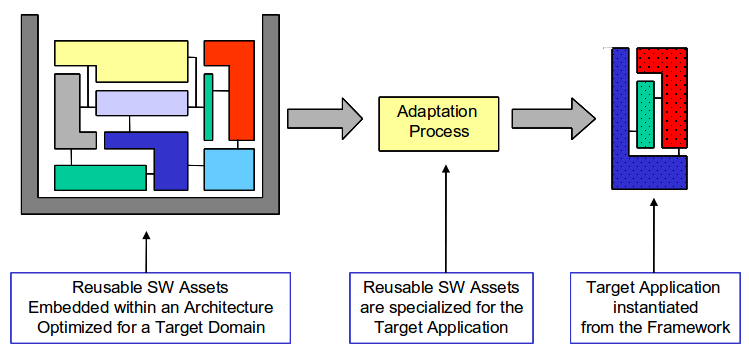
\includegraphics[scale=0.45,keepaspectratio=true]{../images/SwFrameworks.png}
 % PRD.png: 474x227 pixel, 72dpi, 16.72x8.01 cm, bb=0 0 474 227
 \caption{The Software Framework Concept}
 \label{fig:SwFwConcept}
\end{figure}

The FW Profile supports the specification of software frameworks through the concepts of \textit{Adaptation Point} and \textit{Invariant Property}. An Adaptation Point is a point where the behaviour of a pre-defined component offered by the software framework can be modified to meet the needs of a target application. An Invariant Property is a property that is guaranteed to hold on all applications instantiated from the framework. Thus, an invariant property expresses an aspect of the behaviour of the framework that remains unchanged even after the framework components have been adapted for the target application.

The concept of adaptation point supports the specification of software frameworks because the distinguishing characteristic of a framework component (as opposed to a component which is intended for use in a single application) is its adaptability, namely its ability to be modified to match the needs of several related applications. Hence, specification of a framework requires the ability to specify adaptability. The Adaptation Point concept of the FW Profile fulfills this need.

In the FW Profile, adaptability is supported by allowing certain elements of the State Machine and Procedure models to be marked as “adaptation points”. The objective of adaptability in the specification of a software framework is to cover the variability within the framework domain. Adaptability must therefore be controlled to remain limited at a specific domain. For this purpose, the FW Profile imposes restrictions on the type of elements which can be marked as adaptation points. These restrictions are defined so as to allow the definition of invariant properties for a framework.

The role of the invariant properties in the framework instantiation process is illustrated in
figure \ref{fig:InvariantProperties}. The framework is specified to encapsulate the properties that are invariant within its domain (i.e. the properties that must be satisfied by all applications that can be instantiated from the framework). The instantiation process (namely the adaptation of the framework components) guarantees that these properties are preserved at application level and application developers can therefore concentrate on adding their own application-specific properties and can assume that framework-level properties remain satisfied. 

The adaptation mechanisms offered by the FW Profile are discussed further in section \ref{sec:procAdaptation} for Procedures and in section \ref{sec:stateMachineAdaptation} for state machines.

\begin{figure}[H]
 \centering
 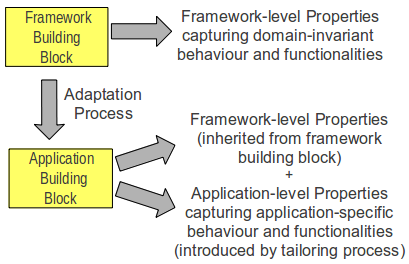
\includegraphics[scale=0.45,keepaspectratio=true]{../images/FW_Adaptation.png}
 % PRD.png: 474x227 pixel, 72dpi, 16.72x8.01 cm, bb=0 0 474 227
 \caption{Invariant Properties}
 \label{fig:InvariantProperties}
\end{figure}

\subsection{Support for Formal Verification}
The FW Profile allows the requirements of an application to be expressed through a complete and unambiguous model of a target application. This in principle allows formal verification techniques to be used to validate the model (i.e. to prove that the model actually satisfies certain properties). This issue is discussesd at greater length in section \ref{sec:formalVerification}.


%====================================================================================
\section{The Procedure Model}
Procedures are one of the three modelling concepts offered by the FW Profile (see section \ref{sec:basicConcepts}).
This section defines the procedure model of the FW Profile. The procedure semantics defined
in this section can be mapped to a subset of the semantics of the activity concept in UML 2.

\subsection{Role of Procedures}
Together with the twin concept of state machines (see next section), procedures are intended to
capture the functional behaviour of an application (see section \ref{sec:funcAndNonFuncBehaviour}). To some extent, state
machines and procedures are interchangeable in the sense that the same abstract behaviour can
often be modelled using either one or the other of these two concepts.
Procedures are, however, especially well-suited to modelling self-contained behaviour, namely
behaviour that is started by some external command but which then continues execution
according to an internal logic. Procedures are also better suited at modelling behaviour that
consists of a linear or quasi-linear sequence of actions.

\subsection{Definition of Procedures}
A procedure in the FW Profile consists of the following elements:

\begin{fw_itemize} 
\item One \emph{initial node}
\item One or more \emph{actions nodes} (or actions)
\item One or more \emph{control flows}
\item Zero or more \emph{decision nodes}
\item Zero or more \emph{final nodes}
\item Two \emph{execution counters}
\end{fw_itemize}

The \emph{initial node} is characterized by one control flow which has the initial node as its source
and has either an action node or a decision node as its target.

An \emph{action node} (or action) is characterized by the following elements:

\begin{fw_itemize} 
\item One or more incoming control flows
\item One outgoing control flow
\item The behaviour associated to the action
\end{fw_itemize}

The incoming control flows are control flows that have the action as its target. The outgoing
control flow is a control flow that has the action as its source.

An action represents a single step within a procedure. It encapsulates behaviour that is not
decomposed further within the procedure. The action's behaviour can be defined using natural
language or some formalism (e.g. an “action language”).

A \emph{control flow} is characterized by the following elements:

\begin{fw_itemize} 
\item One source
\item One target (or destination)
\item Zero or one guards
\end{fw_itemize}

The source and the target are either action nodes or decision nodes. Additionally, the initial
node can be the source of a control flow and the final node can be the target of one or
more control flows.

The guard is a specification which evaluates either to TRUE or FALSE and which
has no side effects. If a control flow has no guard attached to it, then this is equivalent to the control flow having a guard which always evaluates to true.

A \emph{decision node} is characterized by the following elements:
\begin{fw_itemize} 
\item One or more incoming control flows
\item Two or more outgoing control flows
\end{fw_itemize}

The incoming control flows are control flows which have the decision node as its target. The
outgoing control flows are control flows which have the decision node as their source.

For control flows issuing from a decision node, the pre-defined “else” guard is available. This
guard returns TRUE if and only if all the other guards attached to control flows issuing from
the same decision node return FALSE.

The \emph{final node} is characterized by one or more incoming control flows (namely control flows
that have the final node as their target). Note that all final nodes are equivalent and therefore it
would be legitimate to allow only one single final node. The option to have more than one is
introduced as a matter of convenience.

The \emph{execution counters} are unsigned integers which are exclusively characterized by their value. The first execution counter is called the \emph{Procedure Execution Counter} and the second one is called the \emph{Node Execution Counter}.

The execution counters of a procedure count the number of times the procedure has
been executed (one counts the number of times the procedure has been executed since it 
was started and the other counts the number of times the procedure has been executed
since its current node was entered). Since procedures will often be executed periodically,
the execution counters can serve as proxies for measuring the elapsing of time.

The following syntactical constraints apply to the definition of the procedure elements:

\begin{fw_itemize} 
\item C1. The control flows out of a decision node must have a guard.
\end{fw_itemize}

The following dynamical constraints must be satisfied when a procedure is executed:
\begin{fw_itemize} 
\item D1. Among the outgoing control flows from a decision node, at least one must have a
guard which evaluates to true;
\item D2. The evaluation of the guards of a control flow must be free of side-effects;
\item D3. The procedure actions and guards must execute in zero logical execution time.
\end{fw_itemize}

The last constraint implies that the behaviour encapsulated by the actions and by the guards
must be purely functional. In practice, this means that actions and guards cannot include time-
dependent behaviour or behaviour that depends on synchronization with other flows of
execution.

The control flow guards and the actions can act as adaptation points (see section \ref{sec:supportForReusability}). For this
purpose, the FW Profile pre-defines a stereotype called $\langle\langle AP \rangle\rangle$ that can be attached to these
elements. The use of the $\langle\langle AP \rangle\rangle$ stereotype only makes sense in the context of a framework
specification. This is discussed further in section \ref{sec:procAdaptation}.

\subsection{Procedure Behaviour}\label{sec:procBehaviour} 
Four operations may be performed on a procedure: (a) the procedure may be \emph{started}; (b) the
procedure may be \emph{executed}; (c) the procedure may be \emph{stopped}; or (d) the procedure may be
\emph{run}.

Procedures are purely reactive: they wait for one of these four operations to be performed upon
them and they only execute a behaviour in response to one of these operations.

Operations are performed in response to \emph{commands}: the command Start triggers the start
operation; the command Execute triggers the execute operation; the command Stop triggers the
stop operation; and the command Run triggers the run operation.

A procedure may be in two states: STOPPED or STARTED. Initially, by default, the procedure
is in state STOPPED. When the procedure is in state STARTED, it has a \emph{current node}. The
current node is either the procedure's initial node or one of its action nodes.

When a procedure is \emph{started}, the following behaviour is executed:
\begin{fw_enumerate} 
\item If the procedure is in state STARTED, then no further action is performed;
\item If the procedure is in state STOPPED, then it is put in state STARTED, its current
node is set equal to its initial node and its execution counters are reset.
\end{fw_enumerate}

When a procedure is \emph{stopped}, the following behaviour is executed:

\begin{fw_enumerate} 
\item If the procedure is in state STOPPED, then no further action is performed;
\item If the procedure is in state STARTED, then it is put in state STOPPED and its current
node is set to an invalid value.
\end{fw_enumerate}

Thus, the Stop and Start commands toggle the state of a procedure and update its current node.
This is shown in the state diagram of Figure \ref{fig:PR_StartStop}.

\begin{figure}[ht]
 \centering
 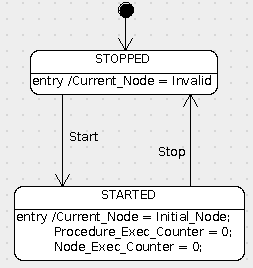
\includegraphics[scale=0.6,keepaspectratio=true]{../images/PR_StartStop.png}
 \caption{Procedure Start/Stop Commands}
 \label{fig:PR_StartStop}
\end{figure}

When a procedure is \emph{executed}, the following behaviour is executed:
\begin{fw_enumerate}
\item If the procedure is in state STOPPED, then no further action is performed;
\item If the procedure is in state STARTED, then its execution counters are incremented
by 1 and the guard attached to the outgoing control flow of the current node is evaluated;
\item If the guard evaluates to FALSE, then no further action is performed;
\item If the guard evaluates to TRUE and the target of the outgoing control flow attached to
the current node is an action node T, then: (a) the current node is set equal to T, (b) the
node execution counter is reset, (c) the
behaviour associated to T is executed, (d) the guard on the out-going control flow of T is evaluated
and steps 3 and 4 are (recusively) repeated;
\item If the guard evaluates to TRUE and the target of the outgoing control flow attached to
the current node is a decision node, then: (a) the guards of the outgoing control flows
attached to the decision node are evaluated; (b) if the target of the outgoing control
flow whose guard evaluates to TRUE is another decision node, then steps (a) to (d) are
performed upon it; (c) if the target of the outgoing control flow whose guard evaluates
to TRUE is an action node T, then the current node is set equal to T, the behaviour
associated to T is executed, the guard on the out-going control flow of T is evaluated
and steps 3 and 4 are (recusively) repeated; (d) if the target of the
outgoing control flow whose guard evaluates to TRUE is a final node, the state of the
procedure is set to STOPPED and the current node is set equal to an invalid value.
\item If the guard evaluates to TRUE and the target of the outgoing control flow attached to
the current node is a final node, then the state of the procedure is set to STOPPED,
and the current node is set equal to an invalid value.
\end{fw_enumerate}

Thus, in summary, when a procedure is executed, it tries to traverse the control flow issuing
form the current node. If this can be done (i.e. if the guard associated to the control flow
evaluates to true), then it advances the execution of the procedure until it finds a guard that
evaluates to false or until it finds a final node. Whenever an action node is traversed, its
associated behaviour is executed.

The Execute command may carry parameters. These parameters may be passed to any of the
actions that are executed as part of the processing of the Execute command.

Note that, at any given time, only one flow of control may be traversing a procedure. This flow
of control is advanced every time that the procedure is executed.

The behaviour associated to the execution of a procedure is shown as an activity diagram in
Figure \ref{fig:PR_Execution}.

\begin{figure}[ht]
 \centering
 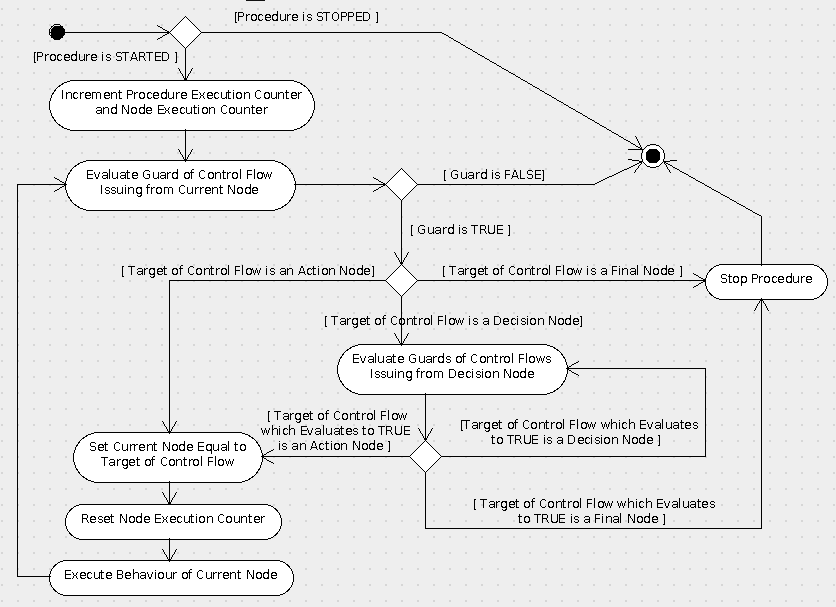
\includegraphics[scale=0.4,keepaspectratio=true]{../images/PR_Execution.png}
 \caption{Procedure Execution Logic}
 \label{fig:PR_Execution}
\end{figure}

Finally, when a procedure is run, the following behaviour is executed:

\begin{fw_enumerate} 
\item The procedure is started;
\item The procedure is executed;
\item The procedure is stopped. 
\end{fw_enumerate}

Thus, the Run operation is defined in terms of the previous three operations. The Run
operation may take parameters which are passed to the Execute operation which is performed
as part of the Run operation (step 2 above).

The Run operation is only useful for procedures which execute in one single cycle. It is
typically used to perform the actions associated to a state in a state machine.

The execution of the various actions associated to the four procedure operations (Start,
Execute, Stop, and Run) is performed in sequence: an action is executed only when the
previous one has completed. Note that, since actions are constrained to execute in zero logical execution
time, the execution of a procedure operation will also execute in zero logical execution time.

Requests to perform an operation upon a procedure are executed in sequence. A new request
can only be processed by a procedure when the previous one has been fully processed.
Procedures have no queues to buffer incoming operation requests.

Note that the procedure operations do not return any values.


\subsection{Specification of Procedure Actions}\label{sec:specProcActions} 
The FW Profile does not mandate any formalism for specifying the behaviour encapsulated in a procedure action. Within a FW Profile Model, a procedure action is typically specified in
terms of the operations which can be performed upon a state machine or upon another procedure.
Thus, examples of typical actions performed by a procedure include:

\begin{fw_itemize} 
\item Starting a procedure
\item Executing a procedure
\item Stopping a procedure
\item Running a procedure
\item Starting a state machine
\item Executing a state machine (i.e. sending an Execute command to it)
\item Sending a transition command to a state machine 
\item Stopping a state machine
\end{fw_itemize}

\subsection{Specification of Procedure Guards}
The FW Profile does not mandate any formalism for specifying a guard. However, it
pre-defines the following guard: “Wait n Cycles”, where n is a positive integer. This guard 
is true only when the node execution counter is greater than or equal to n. 
Thus, this guard implies that the flow of control is held for n
consecutive execution cycles of the procedure.

The case where the procedure has to wait for one cycle (namely where it has to wait for the
next execution) is especially common and for this case the pre-defined guard “Next Execution” may also
be used.

\subsection{Graphical Representation}\label{sec:procGraphRep} 
FW Profile procedures can be conveniently represented using standard UML Activity Diagrams. The mapping from their graphical elements to the elements defined in section \ref{sec:procBehaviour} for the procedures of the FW Profile is the obvious one.

As an example, consider the procedure in figure \ref{fig:PR_Example}. In this figure, when an action consists of performing an operation upon a state machine or upon another procedure (see section \ref{sec:specProcActions}), the following syntax is used: “$\langle operationName \rangle$: $\langle SM\_or\_ProcName \rangle$”. Thus, for instance, if an action consists in starting procedure \texttt{Proc\_A}, the content of the action is expressed as follows: “Start: Proc\_A”.

\begin{figure}[ht]
 \centering
 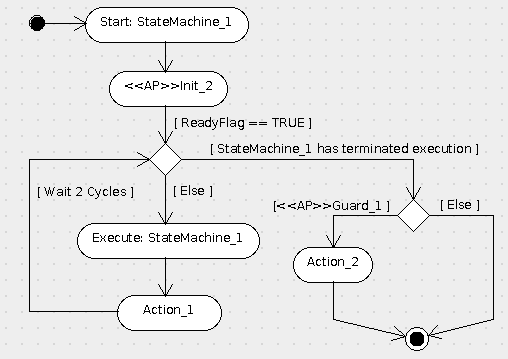
\includegraphics[scale=0.5,keepaspectratio=true]{../images/PR_Example.png}
 \caption{Procedure Example}
 \label{fig:PR_Example}
\end{figure}

After the example procedure of figure \ref{fig:PR_Example} has been started and when it is executed for the first time, the procedure starts the \texttt{StateMachine\_1} state machine and then performs the \texttt{Init\_2} action. Note that these two actions are performed as part of the first execution cycle for the procedure. In fact, if \texttt{ReadyFlag} happens to be true when \texttt{Init\_2} has terminated execution, then, also as part of its first execution cycle, the procedure will evaluate the guards on the top decision node and will proceed along the control flow with a true guard.

After the guard on \texttt{ReadyFlag} has been passed and assuming that \texttt{StateMachine\_1} does not immediately terminate execution, the procedure remains in a loop where it executes the \texttt{StateMachine\_1} and the \texttt{Action\_1} every second execution cycle until the \texttt{StateMachine\_1} terminates. At that point, the procedure itself terminates either immediately or after having executed \texttt{Action\_2}. The choice between these two options (immediate termination or termination after execution of \texttt{Action\_2}) depends on the value of the \texttt{Guard\_1} guard.

The example procedure of Figure \ref{fig:PR_Example} has two adaptation points (see next section): users may adapt this procedure by changing the definition of \texttt{Initi\_2} and/or \texttt{Guard\_1}.

\subsection{Procedure Adaptation}\label{sec:procAdaptation} 
If a procedure is used to specify the behaviour of a framework, then it is necessary to identify its adaptation points (see section \ref{sec:supportForReusability}). The FW Profile relies on the use of the $\langle\langle AP \rangle\rangle$ stereotype to identify adaptable elements within a procedure. 
The FW Profile allows this stereotype to be associated to the following elements:

\begin{fw_itemize} 
\item Actions in Action Nodes
\item Guards on Control Flows
\end{fw_itemize}

The presence of the $\langle\langle AP \rangle\rangle$ stereotype on any of the elements listed above may mean one of two things:

\begin{fw_enumerate} 
\item The content of the stereotyped element is not defined at framework level and the
definition must be done at application level, or
\item A default content for the stereotyped element is defined at framework level but this
can be overridden at application level.
\end{fw_enumerate}

The FW Profile does not provide the means to discriminate between the two cases above.

In section \ref{sec:supportForReusability} it was explained that the adaptation mechanisms supported by the FW Profile are designed to preserve certain invariant properties defined at framework level. What, then, are the properties which are invariant with respect to the adaptation mechanism defined above?

In order to answer this question, it is necessary to consider what \emph{cannot} be modified through the allowed adaptation mechanisms: neither can new nodes or new control flows be added to a procedure, nor can new guards be added to existing control flows. Thus, the features of a procedure which cannot be changed are: (a) the \emph{topology} of the procedure, (b) the \emph{conditions}, expressed in terms of the outcomes of guards, which lead to a control flow being traversed, and (c) the \emph{sequence of actions} which are executed when a control flow is traversed.

The invariant properties of a procedure are therefore those which describe behaviour which depends on the topology of a procedure and on the sequence of control flows traversed and actions performed by the procedure. By contrast, properties which depend on the \emph{content} of the actions or of the guards are typically not invariant since the content of the actions may change during the framework instantiation process.

As an example, consider again the example procedure of the previous section. The following
property holds on the procedure: “\texttt{Action\_1} is executed as many times as 
\texttt{StateMachine\_1} is executed". This property is invariant because it depends merely on the procedure topology and cannot be broken by the adaptation process: all procedures obtained by adapting the procedure of figure \ref{fig:PR_Example} satisfy this property.

Similarly, consider the following property: “if \texttt{StateMachine\_1} is executed,
then the \texttt{ReadyFlag} was true at least once in the past”. This property is invariant because it depends on the topology of the procedure and on the conditions attached to its control flows. Note that \texttt{ReadyFlag} may be undefined at framework level (or it may be defined at framework level but may be overridden at application level) but this does not affect the validity of the property because the property does not depend on the value of the \texttt{ReadyFlag} (which may change during the framework instantiation process) but simply on its presence on a certain transition guard in the procedure (which cannot change during the framework instantiation process the guard is not marked as an adaptation point).

Finally, as an example of a property which is not invariant with respect to the adaptation
mechanisms allowed by the FW Profile, consider the following: “if the procedure executes
\texttt{Action\_1}, then it will also execute \texttt{Action\_2} when it terminates”. This property may hold in some cases (whenever \texttt{Guard\_1} happens to be true) but it is not possible to say whether it holds in all cases because the definition of \texttt{Guard\_1} (which is an adaptation point for the procedure) may be modified during the framework instantiation process.

\subsection{Mapping to Design Level}\label{sec:procMappingToDesignLevel} 
The FW Profile is aimed at the modelling of behaviour. The concepts offered by the FW
Profile to model behaviour can be mapped in many different ways to software-level design
artifacts. In the case of the procedure concept, examples of possible mappings to the software level include:

\begin{fw_itemize} 
\item A procedure is mapped to a single class with an Execute method as execution trigger;
actions and guards are mapped to dedicated methods in the class; adaptation is through inheritance.
\item A procedure is mapped to a single class associated to classes representing its actions 
nodes and guards (a class for each action node or guard); adaptation is through inheritance.
\item A procedure is mapped to a C-style module; actions and guards are mapped to functions 
in the module; adaptation is through delegation.
\end{fw_itemize}

Obviously, the list above is non-exhaustive but the point it tries to make is that the use of the
FW Profile to model the behaviour of an application does not dictate its software-level design.

\subsection{UML 2 Compliance}
The procedure model offered by the FW Profile complies with the UML 2 activity model in
the sense that the elements of the procedure concept of the FW Profile and their semantics can
be mapped in an obvious way to a subset of the elements of the activity concept of UML 2.

The execution counters are specific to the FW Profile. They have been introduced as a
substitute for the concept of time (which does not exist in the FW Profile Procedures): 
if a procedure is executed periodically, then the value of its execution 
counters is proportional to the time elapsed since the procedure was started (Procedure
Execution Counter) or since the current node was entered (Node Execution Counter). 

It should be emphasized that the procedure model proposed by the FW Profile is far more
restrictive than the activity model supported by UML 2. This is because the FW Profile uses
state machines to model purely functional (non-time-related and non-concurrent) behaviour.

\newpage

\section{The State Machine Model}
State machines are one of the three modelling concepts offered by the FW Profile (see section \ref{sec:basicConcepts}). 
This section defines the state machine model of the FW Profile. This model is defined as
a restriction of the state machine model of the UML 2.

\subsection{Role of State Machines}
Together with the twin concept of procedures, state machines are intended to capture the
functional behaviour of an application (see section \ref{sec:funcAndNonFuncBehaviour}). To some extent, state machines and
procedures are interchangeable in the sense that the same abstract behaviour can often be
modelled using either one or the other of these two concepts.

State machines are, however, especially well-suited to modelling reactive behaviour, namely
behaviour that is triggered by external commands. State machines are also better suited at
modelling behaviour that is state-dependent, namely behaviour that is dependent on the past
history of a component or application.


\subsection{Definition of State Machines}\label{sec:smDefinition}
A state machine in the FW Profile consists of the following elements:

\begin{fw_itemize} 
\item One \emph{initial pseudo-state}
\item One or more \emph{states}
\item One or more \emph{state transitions}
\item Zero or more \emph{choice pseudo-states}
\item Zero or more \emph{final pseudo-states}
\item Two \emph{execution counters}
\end{fw_itemize}

The \emph{initial pseudo-state} is characterized by one transition which has the initial pseudo-state as
its source and has either a state or a choice pseudo-state as its target.

A \emph{state} is characterized by the following elements:

\begin{fw_itemize} 
\item Zero or more \emph{entry actions}
\item Zero or more \emph{do actions}
\item Zero or more \emph{exit actions}
\item Zero or one \emph{embedded state machine}
\item One or more \emph{incoming transitions}
\item Zero or more \emph{outgoing transitions}
\end{fw_itemize}

The state actions represent behaviour which is not decomposed further within the state
machine. Actions' behaviour can be defined using natural language or some formalism (e.g. an
“action language”). An embedded state machine is a state machine that is embedded within the
state. Embedded state machines are defined in the same way and have the same semantics as
other FW Profile state machines. An incoming transition is a state transition that has the state
as its target. An outgoing transition is a state transition that has the state as its source.

A \emph{state transition} is characterized by the following elements:

\begin{fw_itemize} 
\item One \emph{transition source}
\item One \emph{transition target} (or \emph{transition destination})
\item Zero or one \emph{transition trigger} (or \emph{transition command})
\item Zero or one \emph{transition guard}
\item Zero or more \emph{transition actions}
 
\end{fw_itemize}

The transition source and the transition target are either a state or a pseudo-state. The transition
trigger is the command that triggers the execution of the transition. A transition guard is a specification that evaluates either to TRUE or to FALSE and has no side effects. A transition with no guard is equivalent to a transition with a guard which always evaluates to TRUE. A transition action represents behaviour which is not decomposed further within the state machine. A transition action behaviour can be defined using natural language or some formalism (e.g. an “action language”).

Transition commands may carry parameters and may return values. The parameters and return
values are not defined further by the FW Profile. They represent parameters that are passed to
the actions and guards and values that are returned by the actions.

A \emph{choice pseudo-state} is characterized by the following elements:

\begin{fw_itemize} 
\item One or more \emph{incoming transitions}
\item One or more \emph{outgoing transitions}
\end{fw_itemize}

An incoming transition is a state transition that has the choice pseudo-state as its target. An
outgoing transition is a state transition that has the choice pseudo-state as its source.

For transitions issuing from a choice pseudo-state, the pre-defined “else” guard is available.
This guard returns TRUE if and only if all the other guards attached to transitions issuing from
the same choice pseudo-state return FALSE.

The \emph{final pseudo-state} is characterized by one or more incoming transitions (namely state
transitions that have the final pseudo-state as their target). Note that all final pseudo-states are
equivalent and therefore it would be legitimate to allow only one single final pseudo-state. The
option to have more than one is introduced as a matter of convenience.

The \emph{execution counters} are unsigned integers which are characterized by their value.
The first execution counter is called the \emph{State Machine Execution Counter} and the second one
is called the \emph{State Execution Counter}.

The following syntactical constraints apply to the definition of the state machine elements:

\begin{fw_itemize} 
\item C1. The same pseudo-state cannot be both source and target for a transition;
\item C2. The source and target of a transition cannot both be choice pseudo-states;
\item C3. The transition that has the initial pseudo-state as source can have neither a guard nor a trigger;
\item C4. Deleted;
\item C5. Transitions that have a choice pseudo-state as source cannot have a transition trigger;
\item C6. Deleted;
\item C7. Transitions that have a state as a source must have a transition trigger;
\item C8. Transitions can only link states and/or pseudo-states that belong to the same state machine.
\end{fw_itemize}

The last constraint implies that transitions from an outer state machine to an embedded state
machines or vice-versa are not allowed. Note, however, that the same transition command may
trigger a transition both in an outer state machine and in one of its embedded state machine.
This is discussed in the next section.

The following dynamical constraints must be satisfied when a state transition is executed:

\begin{fw_itemize} 
\item D1. Among the outgoing transitions from a choice pseudo-state, at least one must have a
guard which evaluates to true;
\item D2. The evaluation of the guards of a transition must be free of side-effects.
\item D3. The state
actions (entry, do, and exit actions) and the transition actions and guards must execute
in zero logical execution time.
\end{fw_itemize}

The last constraint implies that the behaviour encapsulated by actions and guards is
constrained to be \emph{purely functional}. In practice, this means that actions and guards cannot
include time-dependent behaviour or behaviour that depends on synchronization with other
flows of executions.

One type of transition command – the \emph{Execute} command – has a special status in that it
triggers the execution of the current state's do-action. The Execute command models the
situation (common in embedded control systems) of a cyclical scheduler periodically
triggering an application and advancing its execution.

As a matter of terminology, when a state machine is sent the Execute command, the state
machine is said to be \emph{executed}.

The execution counters of a state machine count the number of times the state machine has
been executed (one counts the number of times the state machine has been executed since it 
was started and the other counts the number of times the state machine has been executed
since its current state was entered). Since state machines will often be executed periodically,
the execution counters can serve as proxies for measuring the elapsing of time.

The transition guards, the transition actions and the state actions can act as adaptation points
(see section \ref{sec:supportForReusability}). 
For this purpose, the FW Profile pre-defines a stereotype called $\langle\langle AP \rangle\rangle$ that
can be attached to these elements. The use of the $\langle\langle AP \rangle\rangle$ stereotype only makes sense in the
context of a framework specification. This is discussed further in section \ref{sec:stateMachineAdaptation}.

\subsection{State Machine Behaviour}\label{sec:smBehaviour}
Three operations may be performed on a state machine: (a) the state machine may be \emph{started};
(b) the state machine may be sent a \emph{transition command}; or (c) the state machine may be
\emph{stopped}.

State machines are purely reactive: they wait for one of these three operations to be performed
upon them and they only execute some behaviour in response to one of these operations.

A state machine can be either in a \emph{defined state} or in an \emph{undefined state}. A state machine is in a
defined state from the time it has completed the transition out of its initial pseudo-state to the
time it has either completed the transition into one of its final pseudo-states or has been
stopped.

When a state machine is in a defined state, it has a \emph{current state}. The current state is one of the
states of the state machine.

When a state machine is \emph{started}, the following behaviour is executed:

\begin{fw_enumerate}
\item If the state machine is in a defined state, then no further action is taken.
\item If the state machine is in an undefined state, then its execution counters are reset
and the action associated to the transition
out of its initial pseudo-state is executed. If several transition actions are present, they
are executed in the order in which they are listed.
\item If the destination of the transition out of the initial pseudo-state is a choice pseudo-
state, then the guards of the outgoing transitions from the choice pseudo-state are
evaluated and the actions associated to the transition with a guard evaluating to true is
executed. If several transition actions are present, they are executed in the order in
which they are listed.
\item If the destination of the transition out of the initial pseudo-state is a state, then the
current state of the state machine is set equal to that state.
\item If the destination of the transition out of the initial pseudo-state is a choice pseudo-
state and if the selected transition out of the choice pseudo-state has a state as a target,
then the current state of the state machine is set equal to that target state.
\item The entry action of the current state is executed. If several entry actions are present,
they are executed in the order in which they are listed.
\item If the current state has an embedded state machine, then the embedded state machine is
started.
\item If the destination of the transition out of the initial pseudo-state is a choice pseudo-
state and if the selected transition out of the choice pseudo-state has the final pseudo-
state as a target, then the state machine remains in an undefined state.
\end{fw_enumerate}

With reference to point 3, it is noted that at least one of the guards on the outgoing transitions
from a choice pseudo-state is guaranteed to be true because of constraint D1 in the previous
section.

When a state machine is \emph{stopped}, the following behaviour is executed:
\begin{fw_enumerate}
\item If the state machine is in an undefined state, no further action is taken.
\item If the state machine is in a defined state and its current state has an embedded state
machine, the embedded state machine is stopped.
\item The exit action of the current state is executed. If several exit actions are present, they
are executed in the order in which they are listed.
\item The state machine is set to an undefined state.
\end{fw_enumerate}

The logic of the start and stop commands for state machines is shown in Figure \ref{fig:SmStartStop} as two
activity diagrams.

\begin{figure}[ht]
 \centering
 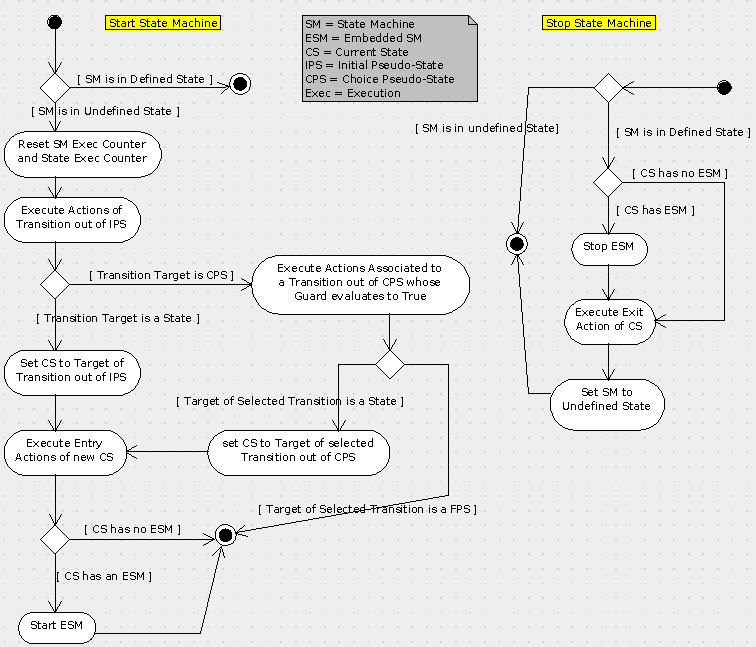
\includegraphics[scale=0.45,keepaspectratio=true]{../images/SM_StartStop.png}
 % PRD.png: 474x227 pixel, 72dpi, 16.72x8.01 cm, bb=0 0 474 227
 \caption{Logic for the Start and Stop Commands to a State Machine}
 \label{fig:SmStartStop}
\end{figure}

When a \emph{transition command T is sent} to a state machine S, then the following behaviour is
executed:

\begin{fw_enumerate}
\item If S is in an undefined state, then no further action is taken.
\item If T is the Execute command, then the execution counters of the state machine are
incremented and the do-action associated to the current state of S is
executed. If several do-actions are present, they are executed in the order in which
they are listed.
\item If S is in a defined state and the current state of S has an embedded state machine SE,
then the transition command T is propagated to SE.
\item If there are no transitions from the current state of S that have T as their trigger, then
no further action is taken.
\item If there are one or more transitions from the current state of S that have T as their
trigger, then their guards are evaluated in sequence. The order of the evaluation is
undefined. The absence of a guard is equivalent to a guard that returns TRUE.
\item When the first transition is found whose guard evaluates to TRUE, then that transition
is executed.
\end{fw_enumerate}

The logic that governs the processing of a transition command by a state machine is shown in
Figure \ref{fig:SmCmdProcessing} as an activity diagram. Note that this logic merely describes the circumstances
under which a transition within a state machine is executed but it does not define the logic
according to which the transition is executed. This is done below (see also Figure \ref{fig:SmTransitionExecution}).

\begin{figure}[ht]
 \centering
 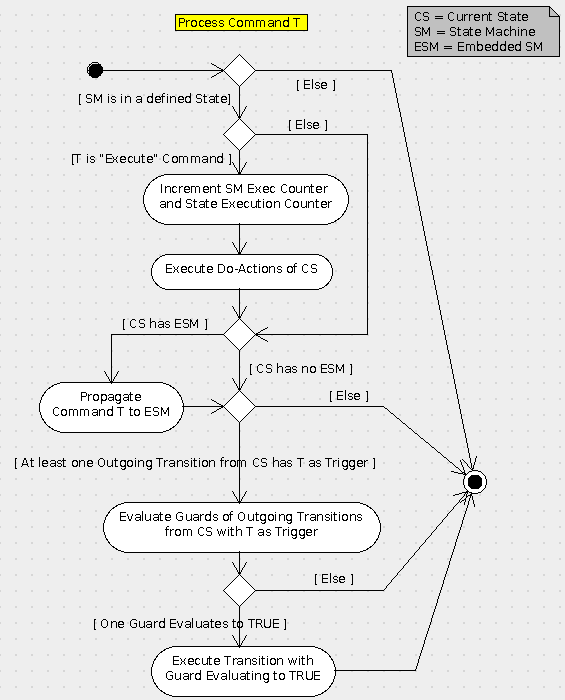
\includegraphics[scale=0.55,keepaspectratio=true]{../images/SM_CmdProcessing.png}
 % PRD.png: 474x227 pixel, 72dpi, 16.72x8.01 cm, bb=0 0 474 227
 \caption{Logic for Processing Transition Commands by a State Machine}
 \label{fig:SmCmdProcessing}
\end{figure}

When a \emph{transition is executed}, then the following behaviour is executed:
\begin{fw_enumerate}
\item If the source state of the transition is a state and that state has an embedded state
machine, then the embedded state machine is stopped.
\item If the source state of the transition is a state, then the exit action associated to the
source state is executed. If several exit actions are present, they are executed in the
order in which they are listed.
\item The transition action associated to the transition is executed. If several transition
actions are present, they are executed in the order in which they are listed.
\item If the target of the transition is a choice pseudo-state, then the guards of the out-going
transitions from the choice pseudo-state are evaluated in sequence until one is found
that evaluates to true and that transition is executed.
\item If the target of the transition is a final pseudo-state, then the state machine is set to an
undefined state and no further action is taken.
\item If the target state of the transition is a state, then the current state of the state machine
is updated to be equal to the target state of the transition and the state execution counter is
reset.
\item If the target state of the transition is a state, then the entry action of the target state is
executed. If several entry actions are present, they are executed in the order in which
they are listed.
\item If the target state of the transition is a state and that state has an embedded state
machine, then the embedded state machine is started.
\end{fw_enumerate}

With reference to point 4, it is noted that at least one of the guards on the outgoing transitions
from a choice pseudo-state is guaranteed to be true because of constraint C6 in the previous
section.

The logic according to which a transition is executed is shown as an activity diagram in Figure \ref{fig:SmTransitionExecution}. 
Note that this logic is called up by the logic shown in the activity diagram of Figure \ref{fig:SmCmdProcessing}.

\begin{figure}[ht]
 \centering
 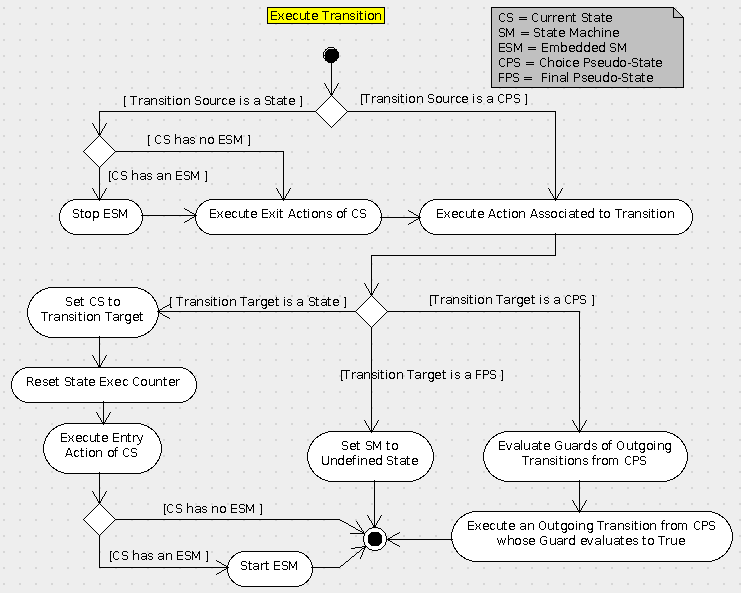
\includegraphics[scale=0.45,keepaspectratio=true]{../images/SM_TransitionExecution.png}
 % PRD.png: 474x227 pixel, 72dpi, 16.72x8.01 cm, bb=0 0 474 227
 \caption{Logic for Executing Transitions in a State Machine}
 \label{fig:SmTransitionExecution}
\end{figure}

Transition commands may carry parameters. These parameters may be passed to any of the
state or transition actions that are executed as part of the processing of the transition command.

The execution of the various actions associated to the three state machine operations is performed in sequence: an action is executed only when the previous one has completed. Note that, since state and transition actions are constrained to execute in zero logical execution time, the execution of a state machine operation will also execute in zero logical execution time.

Transition commands arrive and are processed in sequence. A new command can only arrive
and be processed by a state machine when the previous one has been fully processed. State
machines have no queues to buffer incoming transition commands.

The above rule in particular implies that transition commands cannot be “nested”, namely the
processing of a transition command by a state machine cannot result in a new command being
sent to the same state machine (\emph{nesting rule}).

As an example where the nesting rule would be violated, consider the following situation. A
first transition command is sent to state machine A that triggers a transition from state A1 to
state A2. The entry action of state A2 sends a second transition command to state machine A.

As a second example of violation of the nesting rule, consider a transition command that is
sent to state machine A that triggers a transition from state A1 to state A2. The entry action of
state A2 sends a new transition command to state machine B. State machine B, as part of its
processing of this command, sends a new transition command to state machine A.

Forwarding of transition commands from one state machine A to another state machine B is
instead allowed provided that neither of the two state machines is embedded in the other one.

Forwarding of transition commands from an embedded state machine to its embedding state
machine or vice-versa is forbidden. This restriction helps to avoid the ambiguities that would
arise when, for instance, the entry action of a state in an embedded state machine triggers a
transition in the embedding state machine.

\subsection{Specification of State and Transition Actions}
Although the FW Profile does not mandate any formalism for specifying the content of a state
or transition action, it offers two mechanisms through which this can be done.

Firstly, a state or transition action can be modelled by a procedure. Note, however, that, since
state and transition actions must execute in zero logical execution time, procedures that specify state
machine actions must execute in one single execution cycle (i.e. they must consist of a
sequence of steps that are executed in one single execution of the procedure).

If a procedure is used to define a state or transition action, then the execution of that action must result in the procedure being started and then executed and its execution must result in the procedure terminating.

Secondly, a state or transition action can be defined in terms of operations performed upon
another state machine or upon a procedure. More specifically, a state or transition action can be
defined to do one of the following:

\begin{fw_itemize} 
\item Start a procedure
\item Execute a procedure
\item Stop a procedure
\item Start a state machine
\item Execute a state machine (i.e. send an execute command to it)
\item Send a transition command to a state machine 
\item Stop a state machine 
\end{fw_itemize}

\subsection{Graphical Representation}
FW State Machines can be conveniently represented using standard UML State Machine
diagrams. The mapping from the graphical elements to the elements defined above for the state
machines of the FW Profile is the obvious one.

As an example, consider the procedure in figure \ref{fig:SmExample}. In this figure, when an action consists of performing an operation upon another state machine or upon a
procedure, the following syntax is used: “$\langle operationName \rangle$: $\langle SM\_or\_ProcName \rangle$”. Thus, for
instance, if an action consists in starting procedure \texttt{Procedure\_A}, the content of the action is
expressed as follows: “Start: Procedure\_A”.

When the example state machine of figure \ref{fig:SmExample} is started, it enters either \texttt{STATE\_1} or \texttt{STATE\_2}, depending on the outcome of the evaluation of \texttt{Guard\_1} and \texttt{Guard\_2} (and note that, by virtue of constraint D1 in section \ref{sec:smDefinition}, at least one of the two guards must be true). If \texttt{STATE\_1} is entered, then the following sequence of actions is executed: \texttt{TransAction\_0}; \texttt{n=0}; \texttt{TransAction\_1}; and \texttt{Entry\_1}. If instead \texttt{STATE\_2} is entered, the following sequence of actions is executed \texttt{TransAction\_0}; \texttt{n=0}; \texttt{Entry\_21}; and \texttt{Entry\_22}.

State \texttt{STATE\_3} can only be entered from \texttt{STATE\_2} in response to command transition \texttt{Trigger\_3}. In \texttt{STATE\_3}, the state machine increases the value of the counter n every time it is executed and as long as \texttt{Guard\_1} remains false. If, for instance, \texttt{Guard\_1} becomes true for the first time when Execute is called for the fourth time, then, at the time the state machine enters state \texttt{STATE\_1}, the value of n is equal to 4.

The state machine terminates execution when it is executed at a time when it is in \texttt{STATE\_1}. If the state machine is stopped before it has terminated execution, it is set to an undefined state without any action being performed.

The use of the AP stereotypes is discussed in the next section.

\begin{figure}[ht]
 \centering
 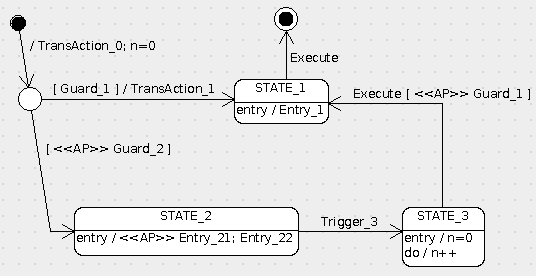
\includegraphics[scale=0.45,keepaspectratio=true]{../images/SM_Example.png}
 % PRD.png: 474x227 pixel, 72dpi, 16.72x8.01 cm, bb=0 0 474 227
 \caption{Example of FW-Compliant State Machine}
 \label{fig:SmExample}
\end{figure}

\subsection{State Machine Adaptation}\label{sec:stateMachineAdaptation} 
If a state machine is used to specify the behaviour of a framework, then it is useful to identify
its adaptation points. The FW Profile offers two adaptation mechanisms for state machines.

The first one relies on the use of the $\langle\langle AP \rangle\rangle$ stereotype (see section \ref{sec:supportForReusability}) 
to identify adaptable elements within a state machine. The FW Profile allows this stereotype to be associated to the
following elements:

\begin{fw_itemize} 
\item Entry Actions
\item Do Actions
\item Exit Actions
\item Transition Actions
\item Transition Guards
\end{fw_itemize}

The presence of the $\langle\langle AP \rangle\rangle$ stereotype on any of the elements listed above may mean one of
two things:

\begin{fw_enumerate} 
\item The content of the stereotyped element is not defined at framework level and the
definition must be done at application level, or
\item A default content for the stereotyped element is defined at framework level but this
can be overridden at application level.
\end{fw_enumerate}

The FW Profile does not provide the means to discriminate between the two cases above.

The second adaptation mechanism allowed by the FW Profile is as follows: if a state does not
have an embedded state machine, then a state machine can be embedded in that state during
the framework instantiation process.

In section \ref{sec:supportForReusability} it was explained that the adaptation mechanisms supported by the FW Profile are
designed to preserve certain invariant properties defined at framework level. What, then, are
the properties which are invariant with respect to the two adaptation mechanisms defined
above?

In order to answer this question, it is necessary to consider what \emph{cannot} be modified through
the allowed adaptation mechanisms: neither can the transition commands be changed, nor can
new actions or new guards be added to existing states or transitions, nor can new states or new
pseudo-states be added to the state machine. Thus, the features of a state machine that cannot
be changed are: (a) the topology of the state machine, (b) the conditions, expressed in terms of
the outcomes of guards, that lead to a state transition taking place, and (c) the sequence of
actions which are executed when a transition is performed.

The invariant properties of a state machine are therefore those which describe behaviour which
depends on the topology of a state machine and on the sequence of transitions and actions
performed by the state machine.

\begin{figure}[ht]
 \centering
 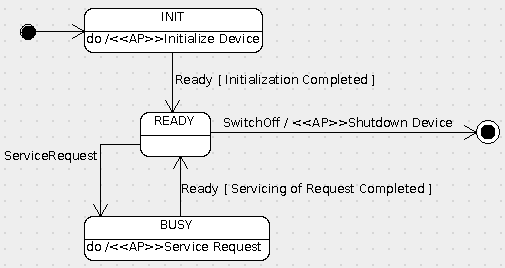
\includegraphics[scale=0.45,keepaspectratio=true]{../images/HwDeviceWithBusyWait.png}
 % PRD.png: 474x227 pixel, 72dpi, 16.72x8.01 cm, bb=0 0 474 227
 \caption{Hardware Device with a Busy Wait}
 \label{fig:HwDeviceWithBusyWait}
\end{figure}

As an example, consider the state machine of figure \ref{fig:HwDeviceWithBusyWait}. This represents a family of hardware devices which can be initialized and shutdown and which, while operational, are capable of servicing requests from their users. The initialization, shutdown and servicing procedures vary across the family of devices and are therefore modelled as adaptation points. The operation logic of the device is instead common to all devices in the family and it is captured in the topology of the state machine. 

Examples of invariant properties for this state machine are: (a) a device can only service a user request, if, at the time the request is made, it is in state READY; (b) a device only executes its shutdown procedure if it is switched off when it is state READY. These properties are invariant because they will hold irrespective of how the adaptation points in the state machine are filled at application level. These properties will also continue to hold if the application designer adds behaviour to the INIT, READY or BUSY states by embedding new state machines into them.

Consider instead the following property: when a device receives the \texttt{Ready} command, it enters the READY state. This property may hold on some devices (depending on how the device is commanded and on how its initialization and request servicing procedures are implemented) but it is not guaranteed by the state machine diagram of figure \ref{fig:HwDeviceWithBusyWait} and should therefore not be relied upon when designing a generic framework.

Figure \ref{fig:SmAdaptation} illustrates the general concept of property invariance for state machines. The
figure shows a base state machine that is extended with the addition of a new embedded state
machine and, possibly, with re-definitions of some of its actions or guards (not shown
explicitly in the figure). The embedded state machine can be used to endow the derived state
machine with additional (application-level) properties but it cannot violate the properties
inherited from the framework level.

\begin{figure}[ht]
 \centering
 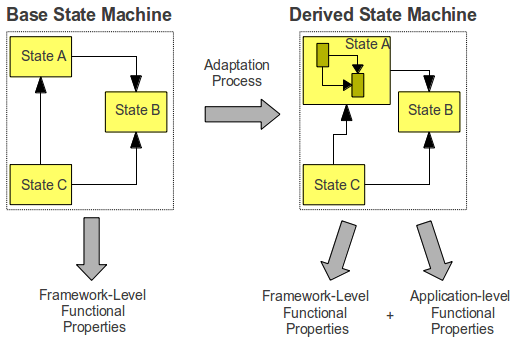
\includegraphics[scale=0.45,keepaspectratio=true]{../images/SM_Adaptation.png}
 % PRD.png: 474x227 pixel, 72dpi, 16.72x8.01 cm, bb=0 0 474 227
 \caption{State Machine Adaptation Process}
 \label{fig:SmAdaptation}
\end{figure}

\subsection{Mapping to Design Level}
The FW Profile is aimed at the modelling of behaviour. The concepts offered by the FW
Profile to model behaviour can be mapped in many different way to software design-level
artifacts. In the case of the state machine concept, the following mappings would be possible:

\begin{fw_itemize} 
\item A state machine is mapped to a single class; the transition triggers and all the actions
and guards are mapped to methods in the class; adaptation is through inheritance.
\item A state machine is mapped to a single class associated to classes representing its states 
(a class for each state); the transition triggers and all the actions and guards are 
mapped to methods in the class; adaptation is through inheritance.
\item A state machine is mapped to a C-style module; the transitions are controlled by a 
single function in the module (a transition is identified by an argument to the 
function); actions and guards are mapped to functions in the module; adaptation is 
through delegation. 
\end{fw_itemize}

Obviously, the list above is non-exhaustive but the point it tries to make is that the use of the
FW Profile to model the behaviour of an application does not dictate its software-level design

\subsection{UML 2 Compliance}
The state machine model offered by the FW Profile complies with the UML 2 state machine
model in the sense that the elements of the state machine concept of the FW Profile and their
semantics can be mapped in an obvious way to a subset of the elements of the state machine
concept of UML 2 with the following provisos:

\begin{fw_itemize}
\item The semantics of choice pseudo-states in the FW Profiles subsumes that of junction pseudo-states
in UML2. Thus, in the FW Profile, choice pseudo-states can also be used to join together incoming
transition flows.
\item The execution counters are specific to the FW Profile. They have been introduced as a
substitute for the concept of time (which does not exist in the FW Profile State Machines):
if a state machine is executed periodically, then the value of its execution 
counters is proportional to the time elapsed since the state machine was started (State Machine
Execution Counter) or since the current state was entered (State Execution Counter). 
\end{fw_itemize}

It should be emphasized that the state machine model proposed by the FW Profile is far more
restrictive than that supported by UML 2. This is because the FW Profile uses state machines
to model purely functional (non-time-related, non-concurrent) behaviour.

\newpage

\section{RT Containers}
RT Containers are one of the three modelling concepts offered by the FW Profile (see section
\ref{sec:basicConcepts}). This section defines the RT Container concept of the FW Profile.

Note that, unlike state machines and procedures (the other two modelling concepts offered by
the FW Profile), RT Containers are not derived from a UML 2 concept.

\subsection{Role of RT Containers}
State machines and procedures allow all functional aspects of a software application to be
modelled. RT Containers complement them by offering a means to capture one aspect of the
time-related behaviour of an application.

It is important to stress that full modelling of an application's timing behaviour is beyond the
scope of the FW Profile. This is because the FW Profile is aimed at modelling individual
applications. Applications normally run on a software/hardware platform which they share
with other applications. Timing behaviour is a system-level aspect (it depends, for instance, on
the relative priorities of the threads allocated to the various applications in a system) and
cannot therefore be fully captured at application level.

RT Containers provide a way to encapsulate the activation logic for a functional behaviour.
More specifically, a RT Container can be seen as a representation of a thread that controls the
execution of some functional behaviour. The RT Container model defined by the FW Profile
allows the conditions under which the thread is released to be specified.

Conceptually, a RT Container can be seen as a software structure that encapsulates some
functional code and endows it with certain timing properties. Thus, RT Containers are a means
of separating the specification of the timing aspects of an application from its functional
aspects.

There is a difference between procedures and state machines on the one hand, and RT Containers on the other hand. All three concepts are offered as means to express the behaviour
of a software application but they exist at different levels of abstraction: state machines and
procedures constitute a generic modelling language for the functional part of an application;
RT Containers allow the timing behaviour of a software application to be modelled but they
presuppose the use of a certain design pattern for handling the activation of functional code.
The RT Container concept is thus less generic than the state machine and procedure concepts.

The design pattern behind the concept of RT Containers is a notification-based model of thread
activation where the notification can be either time-triggered or sporadic (event-driven
notification).

\subsection{Definition of RT Container}
A RT Container is defined by the following elements:

\begin{fw_itemize} 
\item One \emph{Activation Procedure}
\item One \emph{Activation Thread}
\item One \emph{Notification Procedure} 
\end{fw_itemize}

The \emph{Activation Procedure} is a FW Profile Procedure which executes the functional behaviour encapsulated by the RT Container.

The \emph{Activation Thread} is the thread responsible for executing the Activation Procedure (and hence for executing the functional behaviour encapsulated by the RT Container).

The \emph{Notification Procedure} is a FW Profile Procedure which encapsulates the logic for notifying the Activation Thread.

%------------------------------------------------------------------------
\subsection{RT Container Behaviour}\label{sec:rtContainersBehaviour}
Three operations may be performed on a RT Container: (a) the RT Container may be \emph{started}; (b) the RT Container may be \emph{stopped}; and (c) the RT Container may be \emph{notified}.

A RT Container may be in two states: STOPPED or STARTED. Initially, by default, the container is in state STOPPED. When a RT Container is started, the behaviour shown in the activity diagram in the left-hand side of figure \ref{fig:RTStartStop} is executed. The Start operation only has an effect if the container is in state STOPPED when the operation causes the Activation and Notification Procedures to be started and executed once and the Activation Thread to be created and released. The Notification and Activation Procedures are started "atomically" in the sense that neither procedure can be executed or stopped before both have been started. Reference to figure \ref{fig:RTContainerProcedures} shows that the first execution of the Activation and Notification Procedures results in their initialization actions being executed and, in the case of the Activation Procedure, in the first Set-Up Notification action being executed. 

\begin{figure}[ht]
 \centering
 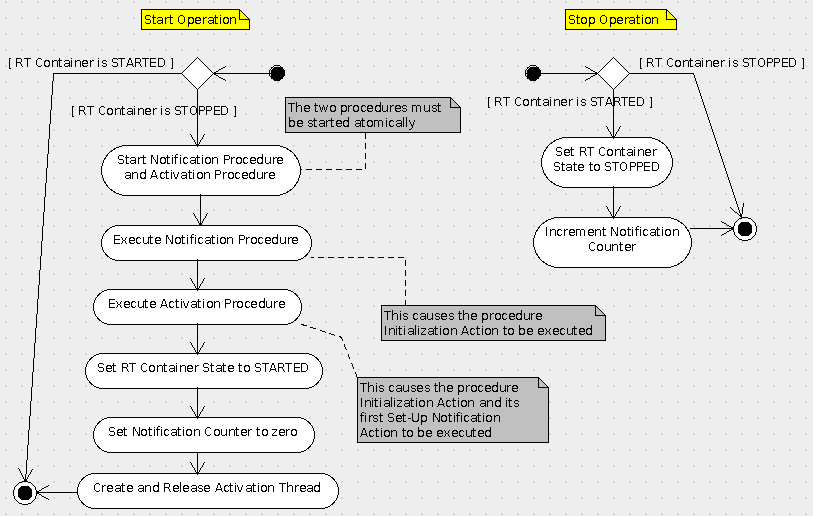
\includegraphics[scale=0.39,keepaspectratio=true]{RTStartStop.png}
 \caption{Start and Stop Operations for RT Containers}
 \label{fig:RTStartStop}
\end{figure}

When a RT Container is stopped, the behaviour shown in the activity diagram in the right-hand side of figure \ref{fig:RTStartStop} is executed. The Stop operation only has an effect if the container is in state STARTED when the operation causes the container to be placed in state STOPPED and the Notification Counter to be incremented. The latter results in one last notification being sent to the Activation Thread. This notification is necessary to ensure an orderly termination of the thread and of the Activation and Notification Procedures. 

When a RT Container is notified, the following behaviour is executed:

\begin{enumerate} 
\item If the RT Container is in state STOPPED, then no further action is performed;
\item If the RT Container is in state STARTED, then its Notification Procedure is executed.
\end{enumerate}

The behaviour of the \emph{Activation Thread} is expressed by the following pseudo-code:

\lstset{language=C,caption={Pseudo-code of Activation Thread},label=code:pseudoCodeActivationThread}
\begin{lstlisting}
while true do {
  wait until Notification Counter is greater than 0;
  decrement Notification Counter;
  execute Activation Procedure;
  
  if (Activation Procedure has terminated) then {
    put RT Container in STOPPED state;
    execute Notification Procedure;
    break;
  }

  if (RT Container is in state STOPPED) then {
    execute Activation Procedure;
    execute Notification Procedure;
    break;
  }
}
\end{lstlisting}

The thread executes a loop which starts with a check on whether there are any pending notifications (the Notification Counter holds the number of pending notifications). If there is a pending notification (i.e. if the Notification Counter is greater than zero), the thread decrements the Notification Counter and then executes the Activation Procedure (which causes the container's functional behaviour to be executed). The thread terminates when the Activation Procedure has terminated or when the RT container has been stopped. In the former case (Activation Procedure has autonomously terminated), the RT Container is put in the STOPPED state and the Notification Procedure is executed one last time before the thread exits; in the latter case (RT Container has been stopped), both procedures are executed one last time. This last execution is intended to give the procedures a chance to perform their finalization behaviour.

\begin{figure}[ht]
 \centering
 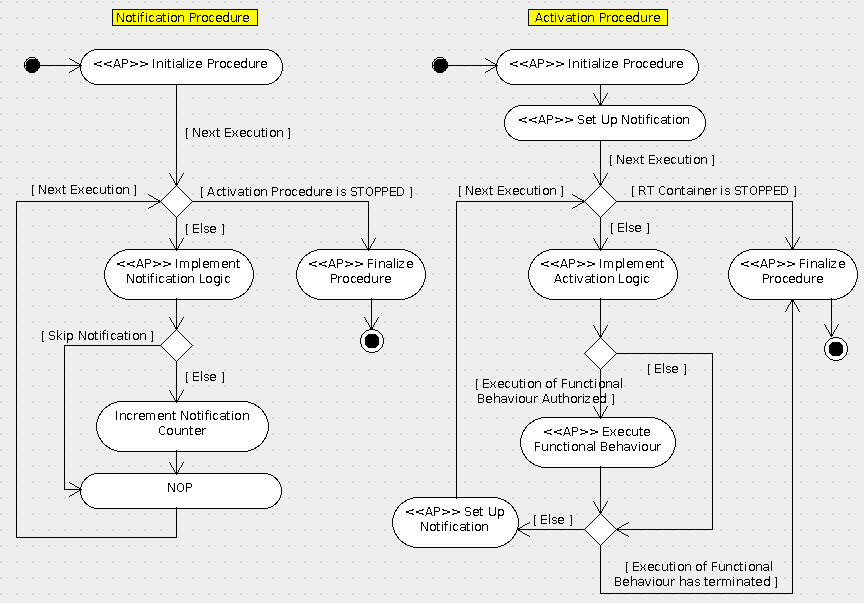
\includegraphics[scale=0.39,keepaspectratio=true]{RTContainer.png}
 % PRD.png: 474x227 pixel, 72dpi, 16.72x8.01 cm, bb=0 0 474 227
 \caption{RT Container Procedures}
 \label{fig:RTContainerProcedures}
\end{figure}

The behaviour of the \emph{Activation Procedure} and of the \emph{Notification Procedure} is shown in the
activity diagrams in Figure \ref{fig:RTContainerProcedures}. The definition of the two procedures makes use of the
“adaptation point” stereotype to identify the parts of the container behaviour which are
application-specific. Applications are therefore expected to extend the two procedures by inserting
their own application-specific behaviour (by contrast, the behaviour of the Activation Thread is invariant and is fully defined at FW Profile level).

When the Activation Procedure is executed for the first time (i.e. after the Activation Thread
has been started), it initializes itself and sets up the first notification of the Activation Thread.
The form of the notification is application-specific. Typically, the setting up of a notification
may consist of one of the following:

\begin{enumerate} 
\item A request that the Activation Thread be notified at some time in the future;
\item A call-back registration to request to be notified when a certain software condition
arises (e.g. a variable changes value, a message arrives, etc);
\item A request to be notified when a hardware interrupt is asserted.
\end{enumerate}

Note that the notification may only need to be set up once when the Activation Procedure is initialized or it may need to be set up at every execution cycle. Note also that the same RT Container may set up different notification requests in the same execution cycle or it may set up notification requests of different kinds at different execution cycles. For this reason, the "Set-Up Notification" in the Activation Procedure is placed both at the beginning of the procedure (to be executed once at initialization time) and inside the loop (to be executed after each execution of the functional behaviour).

When a notification arrives (i.e. when the user of the container executes the Notification Procedure and this increments the Notification Counter), the Activation Thread is woken up and it executes the Activation Procedure. The procedure checks whether the RT Container has been stopped. If this is the case, the procedure performs its finalization action and then terminates. Otherwise, the procedure checks whether the functional behaviour should be executed (this is done by the "Implement Activation Logic" action) and, if so, it executes it. Afterwards, the procedure sets up the next notification (if one is needed) and then checks whether the execution of the functional behaviour has been completed. If this is so, the procedure terminates. Otherwise it waits for the next notification.

The procedure initialization and finalization actions are adaptation points which are defined at application level. Similarly, the action to set up the notification for the Activation Thread and to implement the activation logic must also be defined at application level. The latter could, for instance, be used to implement a filter which decides which notifications to process and which ones to ignore.

The Notification Procedure acts as an intermediary
between the source of the notification event and the notification trigger to the Activation
Thread. Such an intermediary may be useful to: (a) filter notification events, or (b) buffer
notification requests so as to allow the Activation Procedure to handle bursts of notifications.
With reference to the activity diagram in Figure \ref{fig:RTContainerProcedures}, the filtering 
and buffering of notification requests is done in the (application-specific) action “Implement Notification Logic”.

As already noted, the Notification Procedure runs on a thread that is external to the RT
Container: the Notification Procedure is executed by an external thread when the notification
event has occurred. Thus, the logic leading to the notification of the Activation Thread is as
follows:

\begin{fw_enumerate}
\item The Activation Procedure makes a request to be notified when a certain event occurs
(this could, for instance, be done by registering with an external component to be
notified when a certain condition occurs);
\item When the event occurs, the Notification Procedure is executed by the source of the
event;
\item The Notification Procedure evaluates the event and may decide to notify the
Activation Thread;
\item The Notification Procedure notifies the Activation Thread by incrementing the Notification Counter;
\item In response to the notification, the Activation Thread executes the Activation Procedure which may execute the
functional behaviour encapsulated by the RT Container;
\item The Activation Procedure sets up the next notification request.

\end{fw_enumerate}

This cycle is broken when either the Activation Procedure decides that the execution of the
functional behaviour has been completed or when the RT Container is stopped. Either of these
events results in the RT Container and its two procedures terminating.

The Notification Procedure may be executed both by the Activation Thread and by an external thread. For this reason, in many cases, it will be necessary to ensure that it is executed in mutual exclusion.

Note finally that, in this section, the term "event" encompasses both asynchronous occurrences (such as the arrival of hardware interrupts from an external source) or synchronous occurrences (such as periodic signals generated by an operating system). 

%------------------------------------------------------------------------
\subsection{RT Container Properties and Usage Constraints}\label{sec:rtPropUsage}
The RT Container logic defined in the previous section guarantees that certain properties (the \textit{RT Container Properties}) are satisfied when the usage of the RT Container complies with certain constraints (the \textit{RT Container Usage Constraints}). The properties are listed in table \ref{tab:RTContProp} in rows P-3 to P-7. The usage constraints are listed in the same table in rows C-1 to C-3.

\begin{longtable}{|p{0.9cm}|p{10.3cm}|}
\caption{RT Container Properties and Usage Constraints} \label{tab:RTContProp}\\
\hline
\rowcolor{lightblue}
\textbf{N} & \textbf{RT Container Properties and Usage Constraint} \\
\hline\hline
\endfirsthead
\rowcolor{lightblue}
\textbf{N} & \textbf{RT Container Properties and Usage Constraint} \\
\hline\hline
\endhead
P-3 & The Activation Thread shall never deadlock. \\
\hline
P-4 & If the RT Container is stopped after the Activation Thread has been released, then, at some later time, the Activation Procedure shall terminate. \\
\hline
P-5 & If the Activation Procedure stops or terminates (it enters the STOPPED state), then,
at some later time, the RT Container shall be stopped. \\
\hline
P-6 & If the Activation Procedure stops or terminates (it enters the STOPPED state), then,
at some later time, the Notification Procedure shall terminate. \\
\hline
P-7 & Whenever the Activation Procedure is running (it is in state STARTED), then the
Notification Procedure shall be running, too (it shall be in state STARTED). \\
\hline
P-8 & If notifications cease but the RT Container and the Activation Procedure continue to run, then, at some later time, the Activation Thread shall consume all pending notifications (the Notification Counter will become equal to zero). \\
\hline
C-1 & If the RT Container is started and then, at some later time, it is stopped, then it can be re-started only after its Activation and Notification Procedures have terminated
execution and after its Activation Thread has terminated (i.e. the user of a RT Container cannot re-start it before it has completed its orderly shutdown) \\
\hline
C-2 & The Activation Procedure is started, stopped and executed exclusively by the RT
Container (i.e. the user of the container has no access to the Activation Procedure) \\
\hline
C-3 & The Notification Procedure is started and stopped exclusively by the RT Container
itself (i.e. the user of the RT Container can execute the Notification Procedure through the Notify operation but it cannot start or stop it) \\
\hline
\end{longtable}

The usage constraints define the conditions for the legal use of a RT Container. If these
constraints are satisfied, then the user can assume that the RT Container will comply with its
properties. Note that the container's properties hold under all circumstances, irrespective of the
scheduling and notification/triggering policies adopted for the Activation Thread and for the
thread controlling the Notification Procedure and irrespective of the way in which the
adaptation points in the container's procedure are filled.

Properties P-4 and P-5 guarantee that, if the RT Container is stopped or the Activation
Procedure terminates, then the entire container will terminate in the sense that the container
itself and its two procedures will all enter the STOPPED state. 
Property P-8 ensures that, if thread scheduling is fair and the rate at which notifications are generated is compatible with the rate at which they are processed, then no backlog of unprocessed notifications will build up. 

Some notifications may instead remain unprocessed if either the Activation Thread autonomously terminates or the RT Container is stopped by the user. Thus, in informal language, the semantics of the Stop operation on the RT Container is not: "Process all pending notifications and then terminate"; but rather: "Discard any pending notifications and then terminate". 

Note that the container's procedures can only terminate execution “naturally” (as opposed to
being forcefully stopped). This is because the RT Container logic never stops them and usage
constraints C-2 and C-3 ensure that they are not stopped by any external agent. This is
important because it means that the procedure will always execute their finalization behaviour
before terminating.

Constraint C-1 states that a RT Container can only be re-started after it has completed its
shutdown. This is a legitimate constraint because properties P-4 and P-6 guarantee that,
if the container is stopped, then its two procedures will eventually terminate. This means that
the user of a RT Container can always rely on the container completing its shutdown in a finite
amount of time.



The container properties can be formally verified. This is done in table \ref{tab:verifyRT}. The verification
is partially based on the Promela model of the RT Container presented in appendix A.


\begin{longtable}{|p{0.9cm}|p{10.3cm}|}
\caption{Verification of RT Container Properties} \label{tab:verifyRT}\\
\hline
\rowcolor{lightblue}
\textbf{N} & \textbf{Verification of Property} \\
\hline\hline
\endfirsthead
\rowcolor{lightblue}
\textbf{N} & \textbf{Verification of Property} \\
\hline\hline
\endhead
P-3 & Absence of deadlock is verified because the Promela model of appendix A has
no invalid end states. \\
\hline
P-4 & If the following settings are made:
p = “RT Container is in state STOPPED”
q = “Activation Procedure is in state STOPPED” and
z = "Activation Thread has been released";
then property P-4 can be stated in LTL as follows: []((p \&\& z) \textrightarrow$\langle\rangle$q). This property is
satisfied by the Promela model of appendix A (under “weak fairness” conditions). \\
\hline
P-5 & If the same settings are used as for the previous property, then this property can be
stated in LTL as follows: [](!q\textrightarrow[](q\textrightarrow$\langle\rangle$p)). This property is satisfied by the Promela
model of appendix A (under “weak fairness” conditions). \\
\hline
P-6 & If the following settings are made:
p = “Notification Procedure is in state STOPPED” and 
q = “Activation Procedure is in state STOPPED”;
then property P-6 can be stated in LTL as follows: [](q\textrightarrow$\langle\rangle$p). This property is
satisfied by the Promela model of appendix A. \\
\hline
P-7 & If the same settings are used as for the previous property, then this property can be
stated in LTL as follows: [](!q\textrightarrow!p). This property is satisfied by the Promela model of
appendix A. \\
\hline
P-8 & If the following settings are made:
p = “RT Container is in state STARTED",
q = “Activation Procedure is in state STARTED"
u = “No notifications are generated" and
v = “Notification Counter is equal to zero”, 
then this property can be
stated in LTL as follows: $\langle\rangle$[] (u \&\& p \&\& q) \textrightarrow $\langle\rangle$[] v. This property is satisfied by the Promela model of appendix A. \\
\hline
\end{longtable}

\subsection{RT Container Adaptation}
There are no adaptation mechanisms that are specific to RT Containers. RT Containers can be
adapted by adapting their procedures in accordance with the rules of the FW Profile (see
section \ref{sec:procAdaptation}). The adaptation points of a RT Container are the adaptation points of the container's procedures. These are listed in table \ref{tab:rtAdaptPoints}.

\begin{longtable}{|>{\raggedright\arraybackslash}p{3.9cm}|p{7.3cm}|}
\caption{Adaptation Points of RT Containers} \label{tab:rtAdaptPoints}\\
\hline
\rowcolor{lightblue}
\textbf{Adaptation Point} & \textbf{Description} \\
\hline\hline
\endfirsthead
\rowcolor{lightblue}
\textbf{Adaptation Point} & \textbf{Description} \\
\hline\hline
\endhead
Initialize Procedure (Notification Procedure) & Implement the initialization action for the Notification Procedure. \\
\hline
Initialize Procedure (Activation Procedure) & Implement the initialization action for the Activation Procedure. \\
\hline
Implement Notification Logic & Determine whether or not a notification request is forwarded to the Activation Thread. \\
\hline
Set Up Notification & Set up (or update) the mechanism for the next notification. \\
\hline
Implement Activation Logic & Determine whether or not reception of a notification results in execution of the container's functional behaviour. \\
\hline
Execute Functional Behaviour & Execute the container's functional behaviour. \\
\hline
Finalize Procedure (Notification Procedure) & Implement the finalization action for the Notification Procedure. \\
\hline
Finalize Procedure (Activation Procedure) & Implement the initialization action for the Activation Procedure. \\
\hline
\end{longtable}

\subsection{Mapping to Design Level}
As in the case of state machines and procedures, there are many ways in which the behaviour
specified by a RT Containers can be mapped to the design level. Also as in the case of the state machines and procedures, the type of mapping is not mandated by the FW Profile.

%=========================================================================
\section{Formal Verification of FW Profile Models}\label{sec:formalVerification}
The FW Profile offers the means to build a behavioural model of an application. Such a model is developed in response to the needs of a higher-level system within which the application is to be deployed. The question then arises of how one can verify that the model matches the higher-level needs of its embedding system. Traditional answers to this question rely on analysis of the model through reviews by the system's stakeholders. More recently, \textit{formal verification} techniques have been proposed for the same purpose.

Formal verification consists in proving that a certain formally expressed model satisfies certain formally expressed properties. When applied to a requirements model, formal verification techniques are a way of checking the correctness of the requirements: the properties to be verified express the higher-level needs which the requirements are expected to satisfy and formal verification helps establish that the requirements actually do satisfy them (i.e. that the requirements are correct). 

As an example, consider an application which manages a stream of commands to a hardware actuator and which is responsible for controlling its operation. One of the desirable properties of such an application might be to ensure that commands for the actuator never remain pending forever within the application itself (due to, for instance, the actuator having been shut down before the command buffer had been flushed). Establishing at requirements level that this property holds involves analysing the application's requirements to verify that they guarantee that, under all operating conditions, commands are always eventually sent to the actuator. With a formal verification approach this task takes the form of a proof carried out on a formal model of the application's requirements.

Formal verification techniques can be applied whenever requirements are expressed in a formalism with an unambiguous semantics. They can therefore be applied to FW Profile models. The objective of this section is to show how this can be done in practice using a \textit{model checking approach} which is arguably the most common formal verification technique. 

With a model checking approach, compliance of a model to a certain property is verified by systematically exploring all possible states of the model and verifying that, in all cases, the target property is met. Practical use of model checking techniques requires tool support. Here, the Spin Model Checker of reference \cite{ref:spinBook} is considered. This is one of the most widely used model checking tools; it has a strong heritage in industrial projects; and it is publicly and freely available from \cite{ref:spinWebSite}. 

This section thus discusses the applicability of model checking techniques using the Spin Model Checker to FW Profile models. The discussion assumes the reader to be familiar with model checking in general and with the Spin Model Checker in particular.

\subsection{Model-Checking for FW Profile Models}
Figure \ref{fig:FV_BasicApproach} shows the basic approach to model-checking with the FW Profile. The inputs tothe verification process (yellow boxes in the figure) are the FW Profile model itself and the properties which one wishes to verify. The model is translated into an equivalent Promela model and the properties are formalized by being translated into, for instance, LTL formulas or assertions within the Promela code. The Spin Model Checker can then be used to verify whether the properties are satisfied. The outcome of the check is either a confirmation that the properties hold or else an execution trail showing how a certain property is violated.

The appeal of the approach in figure \ref{fig:FV_BasicApproach} is that it would allow the Promela model to be automatically generated from the FW Profile model. Building a tool to translate a model from the FW Profile to the Promela world would be straighforward and would automate the verification process. In reality, this approach would suffer from two major flaws. Firstly, in practical cases, verification is not possible on a \textit{full} model of the target application because the verification would either take too long or exhaust the memory of the computer platform on which it is carried out. Verification must be done on a \textit{reduced} version of the model which only retains the features which are relevant to the properties which are being verified. Secondly, verification of the properties of a certain application normally requires that the environment within which the application is embedded be specified. 

\begin{figure}[h]
 \centering
 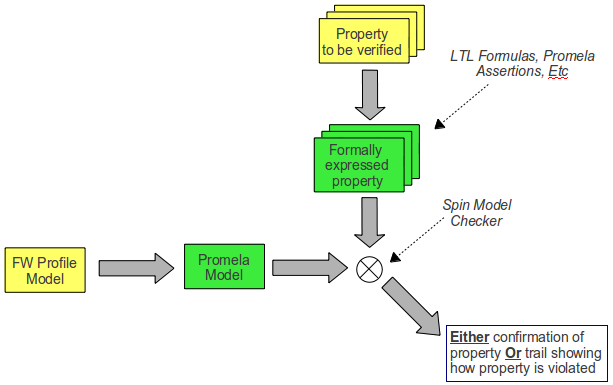
\includegraphics[scale=0.45,keepaspectratio=true]{../images/FV_BasicApproach.png}
 \caption{Basic Approach for Model Cheking of FW Profile Models}
 \label{fig:FV_BasicApproach}
\end{figure}

Thus, a more realistic approach to formal verification is as in figure \ref{fig:FV_RealisticApproach} where the generation of the Promela model requires a "simplification" step which removes all non-relevant features of the FW Profile model and requires, as a second input, the specification of the environment within which the application resides. Automatic generation of the Promela code is still possible but its benefits are much smaller because: (a) the most time-consuming part of the verification process is likely to be the identification of the features to be discarded from the full model; (b) the reduced model must be comparatively simple (or else verification takes too much time or memory) and hence the added value from automating its generation is limited; and (c) the Promela model must cover the application's environment and this cannot be derived automatically from the model of the application requirements.

For all the above reasons, it seems more useful to define general "Promela patterns" of how FW Profile models can be transformed into Promela models rather than to provide a tool which would, at most, only automatize a small part of the transformation. Understanding of these patterns may help a designer to rapidly create Promela models which are adapted to a certain property to be verified. These Promela Patterns are introduced in the next section while section \ref{sec:promelaPatternsExample} presents a concrete example of their use. 

\begin{figure}[ht]
 \centering
 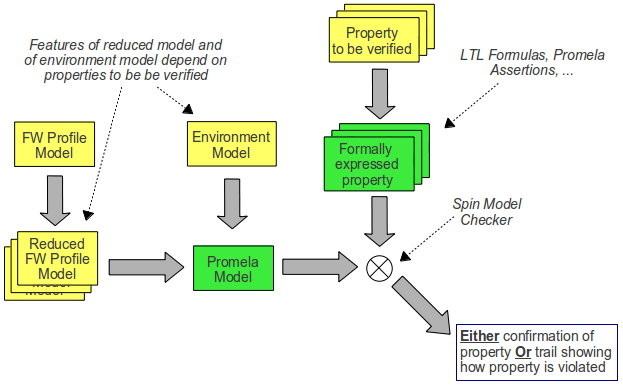
\includegraphics[scale=0.45,keepaspectratio=true]{../images/FV_RealisticApproach.png}
 \caption{Realistic Approach to Model Cheking of FW Profile Models}
 \label{fig:FV_RealisticApproach}
\end{figure}


\subsection{Promela Patterns}
The FW Profile uses state machines and procedures to capture the functional (i.e. purely sequential, non-time related) behaviour of an application and uses RT containers to capture their non-functional behaviour. The basic rules for mapping a FW Profile model to Promela code therefore are:

\begin{fw_itemize}
\item State machines and procedure are mapped to non-blocking code; and
\item RT containers are mapped to Promela processes.
\end{fw_itemize}

The next three sub-sections discuss in greater detail the mapping to Promela of each of the three constructs of the FW Profile.

\subsubsection{State Machines}\label{sec:smPromelaPattern}
This section explains how a FW Profile state machine can be represented in a Promela program. The example Promela listings in this section have been built for the state machine of figure \ref{fig:FV_Buffer}. This state machine represents a buffer controller and is part of the example discussed in section \ref{sec:promelaPatternsExample}.

\begin{figure}[ht]
 \centering
 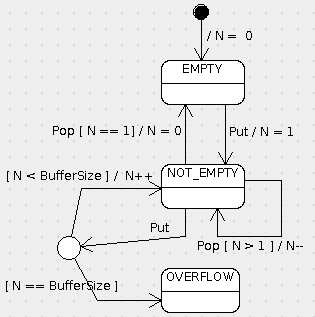
\includegraphics[scale=0.47,keepaspectratio=true]{../images/FV_Buffer.png}
 \caption{State Machine for a Buffer Control Logic}
 \label{fig:FV_Buffer}
\end{figure}

The basic pattern for modelling state machines in Promela is to map them to macros with one single argument representing the start/stop commands and the transition commands for the state machine. For the example state machine, this is illustrated in listing \ref{code:fvSmAsMacros}. The listing begins with the declaration of a set of \texttt{mtype} types which define the set of commands for the state machine and the set of states for the state machine. The set of commands includes both the \texttt{Start}/\texttt{Stop} commands and the transition commands (\texttt{Put} and \texttt{Pop} in the example). The set of states includes an INACTIVE state to represent the situation where the state machine is stopped. 

\lstset{language=Promela,caption={Representation of a State Machine Promela},label=code:fvSmAsMacros}
\begin{lstlisting}
mtype = {INACTIVE};    /* State common to all SMs and Procedures */
mtype = {Start, Stop};             /* Commands common to all SMs */
mtype = {EMPTY, NOT_EMPTY, OVERFLOW};     /* States of Buffer SM */
mtype = {Put, Pop};                     /* Commands of Buffer SM */
mtype bufferState = INACTIVE;              /* State of Buffer SM */
byte nItems = 0;                    /* Number of items in buffer */   

/* ------------------------------------------------------------- */
/* A call to this macro models the sending of a command to the   */ 
/* Buffer State Machine. The buffer size is assumed equal to 3.  */ 
inline BufferSM(cmd) {
   if
   :: (bufferState==INACTIVE) && (cmd==Start) -> 
       bufferState = EMPTY;
       nItems = 0;
   :: (bufferState==EMPTY) && (cmd==Put) -> 
       nItems = 1;
       bufferState = NOT_EMPTY;
   :: (bufferState==NOT_EMPTY) && (cmd==Put) && (nItems<3) -> 
       nItems++;
   :: (bufferState==NOT_EMPTY) && (cmd==Put) && (nItems==3) -> 
       bufferState = OVERFLOW;
   :: (bufferState==NOT_EMPTY) && (cmd==Pop) && (nItems>1) -> 
       nItems--;
   :: (bufferState==NOT_EMPTY) && (cmd==Pop) && (nItems==1) -> 
       nItems = 0;
       bufferState = EMPTY;
   :: (bufferState!=INACTIVE) && (cmd==Stop) -> 
       bufferState = INACTIVE;
   :: else -> skip;
   fi;
} 
. . .
BufferSM(Put);                  /* Send command Put to Buffer SM */
\end{lstlisting}

At line 5, variable \texttt{bufferState} is defined to represent the current state of the state machine. Such a variable is normally initialized to INACTIVE. It may be initialized to a different value if the verification scenario starts with the state machine in an active state.

Obviously, the set of commands in the \texttt{mtype} declarations does not need to encompass \textit{all} commands which the target state machine may accept. Some of these commands may not be relevant to the verification objectives and may be dropped. For the same reason, the declaration of the states may only cover a subset of the state machine's states.

The variable \texttt{nItems} defined at line 6 of the listing matches variable \texttt{N} in the state machine. Variable \texttt{BufferSize} in the example state machine is not directly modelled in the Promela program which simply assumes that the buffer has a size of 3. This choice does not imply any loss of generality since, in a verification context, there is no difference between a situation where the buffer size is equal to 3 and a situation where it has a value greater than 3. This transformation from a variable of arbitrary value to a constant with a well-defined value is an example of the "complexity reduction" step shown in figure \ref{fig:FV_RealisticApproach} .

The macro is defined at lines 11 to 32. A call to this macro represents the sending of a command to the state machine. The macro consists of an \texttt{if} clause which covers all combinations [current state, transition command, guard] which may trigger a transition in the state machine. The combinations of state/command pairs which cannot trigger any transition (or which are simply not relevant to the verification objective) are caught by the \texttt{else} part of the \texttt{if} clause. The behaviour associated to each state/command pair should in principle be the one defined in section \ref{sec:smBehaviour} as the behaviour of a state machine in response to an external command. In practice, aspects of this behaviour which are not relevant to the verification objective should be dropped. Thus, for instance, the example in listing \ref{code:fvSmAsMacros} does not model the execution counters which are associated to each state machine. This is legitimate in the case of the example state machine because none of its guards depends on the passage of time or on the execution cycle of the state machine.

Line 34 shows how the macro is called. In this line, transition command \texttt{Put} is sent to the state machine.

One variant to the code in listing \ref{code:fvSmAsMacros} occurs when the implementation adds a mutual exclusion mechanism in order to let the Buffer state machine be accessed by multiple threads. If the mutual exclusion mechanism is important for verification purposes, it must be modelled in the Promela code. One way of doing this is to associate a boolean variable to the state machine and then to use it as a mutex. The variable is indivisibly tested-and-set at the beginning of the state machine macro (to model the seizing of the mutex) and is reset at the end of the macro (to model the release of the mutex). Listing \ref{code:fvSmAsMacrosWithMutex} shows how this would be done in the case of the Buffer state machine.

The examples of the mutex and of the execution counters (both of which may be included or omitted in a Promela model depending on the verification objective) and the fact that the set of states or of transition commands may be tailored to the verification objectives illustrate how the need may arise to maintain different Promela representations of the same state machines which are aimed at different verification objectives. One way to handle this variability is to put the definition of the state machine macro in a separate file which is then included in the Promela program (using the \texttt{\#include} directive). This lets a user create different versions of the state machine macro which are stored in separate files and have the same calling interface. It then become possible to rapidly switch between alternative representations of the same state machine with minimal impact on the overall Promela program.

\lstset{language=Promela,caption={Representation of a Mutex-Protected State Machine in Promela},label=code:fvSmAsMacrosWithMutex}
\begin{lstlisting}
mtype = {INACTIVE};    /* State common to all SMs and Procedures */
mtype = {Start, Stop};             /* Commands common to all SMs */
mtype = {EMPTY, NOT_EMPTY, OVERFLOW};     /* States of Buffer SM */
mtype = {Put, Pop};                     /* Commands of Buffer SM */
mtype bufferState = INACTIVE;              /* State of Buffer SM */
bool bufferMutex = false;                 /* Mutex for Buffer SM */
byte nItems = 0;                    /* Number of items in buffer */   

/* ------------------------------------------------------------- */
/* A call to this macro models the sending of a command to the   */ 
/* Buffer State Machine. The buffer size is assumed to be equal  */ 
/* to three.                                                     */
inline BufferSM(cmd) {
   atomic{(bufferMutex==false) ->
          bufferMutex = true;}                /* Seize the mutex */
   . . . 
   bufferMutex = false;                     /* Release the mutex */
} 
\end{lstlisting}

\subsubsection{Procedures}\label{sec:prPromelaPattern}
This section explains how a FW Profile procedure can be represented in a Promela program. The example Promela listing in this section has been built for the procedure of figure \ref{fig:FV_ActuatorController}. This procedure controls a hardware actuator and is part of the example discussed in section \ref{sec:promelaPatternsExample}. 

\begin{figure}[ht]
 \centering
 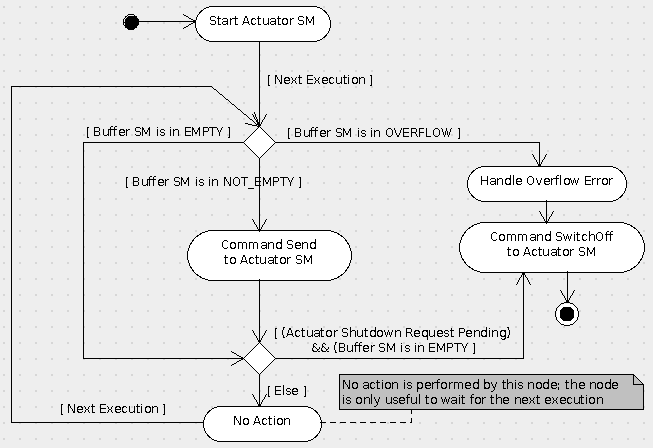
\includegraphics[scale=0.45,keepaspectratio=true]{../images/FV_ActuatorController.png}
 \caption{Procedure to Control a Hardware Actuator}
 \label{fig:FV_ActuatorController}
\end{figure}

The basic pattern for representing procedures in Promela is to split their mapping to Promela into two parts. The first part consists of dedicated code which models the start/stop logic for the procedure. The second part consists of a parameterless macro which models the execution of the procedure. This is illustrated in listing \ref{code:fvPrAsMacros} for the example procedure. 

The listing begins with the declaration of an \texttt{mtype} type which defines the possible states of the procedure. All procedures have a STOPPED and a STARTED state which correspond to the procedure being stopped or having just been started. Additionally, procedures have one state for each node at the end of a control flow with a guard. This state represents the condition of a procedure which is being executed and which has found the guard to be false. The example procedure has two control flows with a guard attached to them but both these control flows end in the same node (the decision node after the "Start Actuator SM" action node) and hence only one additional state needs to be defined for this procedure. In listing \ref{code:fvPrAsMacros} this state is called WAITING. 

The procedure macro consists of an \texttt{if} clause (see lines 7 to 31 in the listing) which covers all states of the procedure and associates to each the behaviour of the procedure when it receives an Execute command in that state. This is in principle the behaviour defined in section \ref{sec:procBehaviour} but, as in the case of the state machine macros, behaviour which is not relevant to the verification can (and should) be dropped. Thus, for instance, the example in the listing does not model the procedure execution counters.

The starting and stopping of the procedure is modelled by setting the procedure state to, respectively, STARTED and STOPPED (see lines 38 and 44 in the listing). The execution of the procedure is modelled by a call to the procedure macro (see lines 40 and 42 in the listing).

As in the case of state machines, there is one obvious variant to the code in listing \ref{code:fvPrAsMacros} which occurs when the implementation adds a mutual exclusion mechanism in order to let the procedure be accessed by multiple threads. If the mutual exclusion mechanism is important for verification purposes, it must be modelled in the Promela code. One way of doing this is to associate a boolean variable to the procedure and then to use it as a mutex. The variable is indivisibly tested-and-set at the beginning of the procedure macro (to model the seizing of the mutex) and is reset at the end of the macro (to model the release of the mutex). The mechanism is the same as for the state machine of listing \ref{code:fvSmAsMacrosWithMutex}.

Also as in the case of state machines, the need to tailor a Promela model to a certain verification objective and to keep it as simple as is compatible with that objective will inevitably result in several models being developed for a given procedure with each model encapsulating different aspects of the procedure's behaviour. One way of handling this variability is to proceed as recommended for the state machines and to give the various versions of the procedure the same calling interface and place them into \texttt{\#include} files which may then be included in the main Promela program. 

\lstset{language=Promela,caption={Representation of a Procedure in Promela},label=code:fvPrAsMacros}
\begin{lstlisting}
mtype = {STOPPED, STARTED, WAITING};  /* Act. Cont. Proc. States */ 
mtype actContState = STOPPED;   /* State of Actuator Cont. Proc. */ 

/* ------------------------------------------------------------- */
/* A call to this macro models the execution of the Actuator     */
/* Controller Procedure.                                         */
inline ActuatorControllerPR() {
   if
   :: (actContState==STOPPED) -> 
       skip;    
   :: (actContState==STARTED) -> 
       ActuatorSM(Start);                   /* Start Actuator SM */  
       actContState = WAITING;
   :: (actContState==WAITING) -> 
       if
       :: (bufferState==EMPTY) -> skip;
       :: (bufferState==NOT_EMPTY) ->
           ActuatorSM(Send);         /* Send Send to Actuator SM */
       :: (bufferState==OVERFLOW) ->
           overflowHandled = true;
           ActuatorSM(SwitchOff);   /* Send SwitchOff to Act. SM */
           actContState = STOPPED;        /* Terminate procedure */
       fi;
       if
       :: (shutdownReqPending==true) && (bufferState==EMPTY) ->
          ActuatorSM(SwitchOff);    /* Send SwitchOff to Act. SM */
          actContState = STOPPED;         /* Terminate procedure */
       :: else -> skip;
       fi;
   fi;
} 
. . .
/* ------------------------------------------------------------- */
/* Promela Process executing Actuator Controller Procedure.      */
active proctype SomeProcess() {
  . . .
  /* Start Actuator Controller Procedure */
  actContState = STARTED;
  . . .
  ActuatorControllerPR();    /* Execute Actuator Cont. Procedure */
  . . .
  ActuatorControllerPR();    /* Execute Actuator Cont. Procedure */
  . . .
  actContState = STOPPED;       /* Stop Actuator Cont. Procedure */
  . . .
}  
\end{lstlisting}

\vspace*{-5mm}
\subsubsection{RT Containers}
This section explains how a RT container can be represented in a Promela program. Mapping of RT containers to Promela can be done at two levels. A detailed mapping requires modelling of the two procedures in the container (the Activation Procedure and the Notification Procedure, see section \ref{sec:rtContainersBehaviour}). In this case, the Promela model in appendix \ref{sec:verificationModelForRtContainers} can be used. 

Such a detailed modelling is, however, unlikely to be necessary. The RT container procedures are designed to guarantee that containers are well-behaved (to guarantee, for instance, that they initialize correctly or that they do not miss any notification requests). Applications will normally take this well-behavedness for granted (because it has been proven at the level of the container) and will instead focus on the interaction between the containers and the functional behaviour which they control. A more coarse-grained modelling of the RT containers then becomes more appropriate where a RT container is seen as a source of transition commands to state machines and of execution requests to procedures. In this case, the RT container is simply represented by a Promela process whose body sends the commands and execution requests.

As a simple example, listing \ref{code:fvRtAsProcess} shows a RT container which represents a thread which starts the Buffer State Machine of listing \ref{code:fvSmAsMacros} and then repeatedly sends it \texttt{Put} commands until it eventually stops it. 

\lstset{language=Promela,caption={Representation of a RT Container in Promela},label=code:fvRtAsProcess}
\begin{lstlisting}
active proctype ActuatorHardware() {
  BufferSM(Start);
  do
  :: true -> BufferSM(Put);
  :: true -> break;
  od;
  BufferSM(Stop);
} 
\end{lstlisting}

\subsection{Example Application of Promela Patterns}\label{sec:promelaPatternsExample}
This section illustrates the concepts discussed above to present a complete example of how a FW Profile model can be mapped to a Promela program and how its properties can be verified using the Spin Model Checker. The example problem considered in this section is that of a software controller for a hardware actuator with the following characteristics:  

\begin{fw_enumerate}
\item By default, the hardware actuator is unpowered in the OFF state.
\item The hardware actuator is switched on by sending it command \texttt{SwitchOn}. In response to this command, the hardware actuator performs some internal initialization actions and then enters its normal operational state. 
\item The hardware actuator signals completion of its initialization and entry into its normal operational state by sending a \texttt{Done} signal to its software controller.
\item When it is in its normal operational state, the actuator accepts actuator commands from its controller.
\item The processing of an actuator command takes some time; when the hardware actuator has terminated processing an actuator command, it generates a \texttt{Done} signal to its software controller.
\item The hardware actuator can only process actuator commands one at a time (i.e. there is no internal buffering of commands in the hardware actuator).
\item An orderly switch off of the hardware actuator is performed by sending it command \texttt{SwitchOff} at a time when it is not busy processing an actuator command.
\end{fw_enumerate}

Figures \ref{fig:FV_Actuator} and \ref{fig:FV_ActuatorController2} capture the FW Model of a controller for the hardware actuator. Such a model might be used as a specification for a software module in an embedded control application. The model consists of two state machines (the \textit{Buffer State Machine} and the \textit{Actuator State Machine} in figure \ref{fig:FV_Actuator}) and one procedure (the \textit{Actuator Controller Procedure} in figure \ref{fig:FV_ActuatorController2}).

Since the hardware actuator has no buffering capability for the commands it receives, the Buffer State Machine is introduced to buffer software-level requests for actuator commands. The application sends \texttt{Put} commands to this state machine when it wishes to enqueue an actuator command. The buffer has two nominal states (EMPTY and NOT\_EMPTY) and one error state (OVERFLOW) which is entered when the rate at which the application makes actuator command requests is greater than the rate at which the hardware actuator can process them.

The Actuator State Machine controls the hardware actuator. When the state machine is started, it sends a \texttt{SwitchOn} command to the hardware actuator and it starts the Buffer State Machine. It then waits in state INIT until the hardware actuator confirms that it has completed its initialization by issuing a \texttt{Done} command (in practice, this command would originate from an interrupt processing routine which is triggered by the \texttt{Done} signal generated by the hardware actuator). After initialization, the Actuator State Machine enters state READY where it waits for a \texttt{Send} command which triggers the collection of a command from the Buffer and its forwarding to the hardware actuator. While the hardware actuator is busy processing a command request, the Actuator State Machine remains in state BUSY and returns to state READY when the hardware actuator sends it a \texttt{Done} command to signal its readiness to process the next command. When the state machine is in state READY, it may be switched off. This causes a \texttt{SwitchOff} command to be sent to the hardware actuator and the Buffer State Machine to be stopped.

The Actuator Controller Procedure of figure \ref{fig:FV_ActuatorController2} controls the operation of the two state machines and, through them, of the hardware actuator. Initially, both state machines are inactive. When the application wishes to start using the hardware actuator, it starts the Actuator Controller Procedure. This causes the Actuator State Machine to be started and (indirectly) the Buffer State Machine to be started. Subsequently, the application periodically executes the procedure. At each execution, the procedure checks whether there are any pending commands in the buffer and, if so, it triggers the Actuator State Machine to process them. The procedure can terminate either nominally (if there has been a shutdown request for the actuator) or abnormally (if the command buffer has overflown).  

Table \ref{tab:actContProp} lists four desirable properties which a well-designed actuator controller should satisfy. The list is of course not exhaustive but it gives an idea of the kind of properties for which a formal verification approach might be useful.  

\newpage
\begin{longtable}{|p{0.9cm}|p{10.3cm}|}
\caption{Properties of Actuator Controller} \label{tab:actContProp}\\
\hline
\rowcolor{lightblue}
\textbf{N} & \textbf{Property Definitio} \\
\hline\hline
\endfirsthead
\rowcolor{lightblue}
\textbf{N} & \textbf{Property Definition} \\
\hline\hline
\endhead
P-1 & Pending commands in the buffer are always eventually sent to the hardware actuator. \\
\hline
P-2 & If the Actuator State Machine is inactive, then the Buffer State Machine is inactive too. \\
\hline
P-3 & If a shutdown request is made, then, eventually, the entire actuator function is shut down. \\
\hline
P-4 & Buffer overflows are always eventually handled. \\
\hline
\end{longtable}

The Promela program which was used to verify the properties in the table is listed in full in appendix \ref{sec:promelaProgForActExample}. The bulk of the program consists of three macros which represent the two state machines and the procedure of the actuator function. Their structure is in line with the patterns presented in sections \ref{sec:smPromelaPattern} and \ref{sec:prPromelaPattern}. 

The application within which the actuator function is embedded is represented by process \texttt{ApplicationSoftware}. This process defines how the application uses the actuator function. The model in the Promela program assumes that the application initially starts the Actuator Controller Procedure and then sends a sequence of command requests to the Buffer State Machine interleaved with a sequence of execution requests to the Actuator Controller Procedure until, eventually, a shutdown request is made to stop operation of the hardware actuator.

The hardware actuator is modelled as a second process \texttt{HardwareActuator} which implements the behaviour defined in the bulleted list at the beginning of this section. In terms of the terminology of figure \ref{fig:FV_RealisticApproach}, the \texttt{ApplicationSoftware} and the \texttt{HardwareActuator} processes represent the "environment" around the behaviour which must be verified.

The properties listed informally in table \ref{tab:actContProp} are formalized at the end of the Promela program in appendix \ref{sec:promelaProgForActExample} as LTL formulas which are then used by the Spin Model Checker as positive forms of \texttt{never} claims. As stated in the program, only the last property P-4 is satisfied. Properties P-1 to P-3 are \textit{not} satisfied. This fact is somewhat counter-intuitive and deserves some discussion to highlight the importance of a formal verification approach.

Property P-1 ("Pending commands in the buffer are always eventually sent to the hardware actuator") is formalized as follows:

% The next listings should have no caption 
\captionsetup[lstlisting]{labelformat=empty,labelsep=none}

\lstset{language=Promela,caption={},label=code:fvP1}
\begin{lstlisting}
#define p (actReqDone==false) /* No Put request to Buffer is done*/
#define q (nItems==0)         /* No pending items in Bufer       */

/* If no new commands are placed in the buffer, then, eventually,*/
/* all pending commands are sent to the actuator.                */
ltl P1 {(<>[]p) -> (<>[]q)}
\end{lstlisting}

One would expect this property to be violated exclusively when, at the time the actuator function is shut down, there are some pending commands left in the buffer. The property would thereore seem to be guaranteed by the fact that the Actuator Controller Procedure only services a shutdown request if the buffer is empty (i.e. if all pending  actuator commands have been processed). In reality, the Spin Model Checker shows that a violation may arise in the following scenario:

\begin{fw_itemize}
\item The hardware actuator is switched on and is initializing.
\item The Actuator State Machine is in state INIT and the Buffer State Machine is in state EMPTY.
\item A shutdown request is made by the application. 
\item Since the buffer is empty, the Shutdown request is serviced at the next execution of the Actuator Controller Procedure which sends a \texttt{SwitchOff} command to the Actuator State Machine and then terminates.
\item Since the Actuator State Machine is still in state INIT, the \texttt{SwitchOff} command has no effect and both it and the Buffer State Machine remain active.
\item Some time later, a command is deposited in the buffer and remains permanently pending - this violates property P-1.
\end{fw_itemize}

Violation of the property could probably be avoided either by constraining the application not to shut down the actuator function while initialization is under way; or by modifying the Actuator State Machine to respond to \texttt{SwitcOff} commands when it is in the INIT state.

Property P-2 ("If the Actuator State Machine is inactive, then the Buffer State Machine is inactive too") is formalized as follows:

\lstset{language=Promela,caption={},label=code:fvP1}
\begin{lstlisting}
#define r (actState==INACTIVE)     /* Actuator SM is inactive    */
#define s (bufferState==INACTIVE)  /* Buffer SM is inactive      */

/* If Actuator SM is inactive, then Buffer SM is inactive too    */
ltl P2 {[](r->s)}
\end{lstlisting}

One would expect this property to be satisfied because the Buffer State Machine is started as part of the starting of the Actuator State Machine and it is stopped as part of its stopping. In fact, the Spin Model Check shows a violation under the following conditions:

\begin{fw_itemize}
\item When the Actuator State Machine is started, the transition action out of its Initial Pseudo State is executed (at this time, the state machine is still in an inactive state).
\item The transition action starts the Buffer State Machine which therefore leaves its inactive state \textit{before} the Actuator State Machine reaches its INIT state. This creates a violation of property P-2.
\end{fw_itemize}

Property P-3 ("If a shutdown request is made, then, eventually, the entire actuator function is shut down") is formalized as follows:

\lstset{language=Promela,caption={},label=code:fvP1}
\begin{lstlisting}
#define r (actState==INACTIVE)     /* Actuator SM is inactive    */
#define s (bufferState==INACTIVE)  /* Buffer SM is inactive      */
#define t (shutdownReqPending==true) /* Shutdown request made    */
#define u (actHwState==OFF)        /* HW Actuator is switched off*/

/* If a shutdown request is made, then, eventually, Actuator SM  */
/* and Buffer SM terminate and Actuator HW is switched off       */
ltl P3 {[](t -> <>[](r && s && u))}
\end{lstlisting}

One would expect this property to be verified because a shutdown request causes the Actuator Controller Procedure to terminate by switching off the Actuator State Machine which in turns triggers commands to switch off the hardware and to stop the Buffer State Machine. In fact, this property is violated for the same reason that property P-1 is violated: if the application makes a shutdown request before the initialization of the hardware actuator has been completed, the hardware actuator will never be switched off.

Finally, property P-4 ("Buffer overflows are always eventually handled") is formalized as follows:

\lstset{language=Promela,caption={},label=code:fvP1}
\begin{lstlisting}
#define v (overflowHandled==true)    /* Overflow error handled  */
#define w (actContExec==true)    /* Act. Cont. PR is executed   */
#define x (actState==READY)         /* Actuator SM is in READY  */
#define y (actState==BUSY)          /* Actuator SM is in BUSY   */
#define z (bufferState==OVERFLOW)   /* Buffer SM is in OVERFLOW */
#define a (actContState==WAITING)    /* Act. Cont. PR is active */

/* If, during normal operation (i.e. after the Actuator has     */
/* completed its initialization and while the Controller        */
/* Procedure is active), the Buffer overflows and then the      */
/* Actuator Controller Procedure executes, then the overflow    */
/* error is handled.                                            */
ltl P4 {[]((z && a && (x || y) && <>w) -> <>v)}
\end{lstlisting}

% Restore captions for listings
\captionsetup[lstlisting]{labelformat=default,labelsep=colon}

This property is satisfied but it should be stressed that it is only satisfied because, in the light of the violations of properties P-1 and P-3, it has been restricted to apply only after the actuator initialization has been completed. If this restriction had been omitted, then the property would have been violated for exactly the same reasons which led to violation of properies P-1 and P-3. 

In summary, this example shows that FW Profile models can be easily and systematically mapped to Promela programs where formal verification of their properties can be performed using the Spin Model Checker.

\newpage
\begin{figure}[ht]
 \centering
 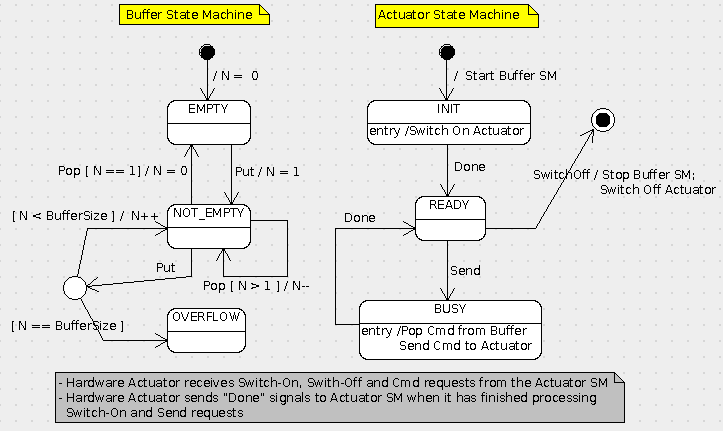
\includegraphics[scale=0.45,keepaspectratio=true]{../images/FV_Actuator.png}
 \caption{State Machines to Control the Hardware Actuator}
 \label{fig:FV_Actuator}
\end{figure}
\begin{figure}[ht]
 \centering
 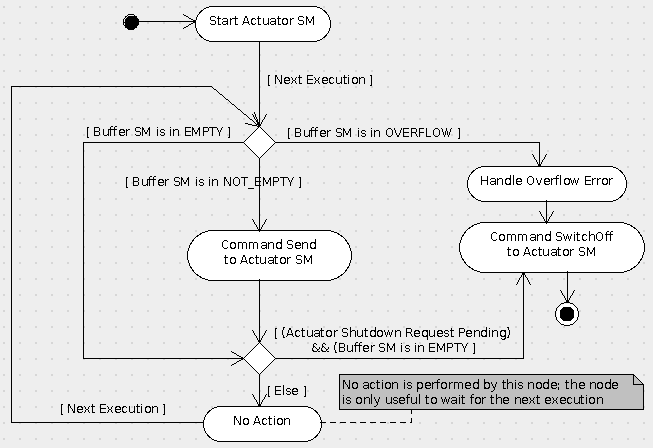
\includegraphics[scale=0.45,keepaspectratio=true]{../images/FV_ActuatorController.png}
 \caption{Actuator Controller Procedure}
 \label{fig:FV_ActuatorController2}
\end{figure}



%=========================================================================
\appendix
\section{Verification Model for RT Container}\label{sec:verificationModelForRtContainers}
This appendix presents the Promela model used to verify the properties of the RT Container defined by the FW Profile (see section \ref{sec:rtPropUsage}).  

\begin{landscape}
\lstset{language=Promela,caption={Verification Model for RT Container},label=code:verificationModelsForRTContainer}
\lstinputlisting[language=Promela]{RTContainer.pml}
\end{landscape}

%------------------------------------------------------------------------
\section{Promela Program for Actuator Control Example}\label{sec:promelaProgForActExample}
This appendix presents the complete Promela program for the formal verification of the actuator control example discussed in section \ref{sec:promelaPatternsExample}. The Promela code includes (at the very end) the definition of the LTL formulas which represent the properties to be satisfied by the actuator controller.   

\begin{landscape}
\lstset{language=Promela,caption={Verification Model for Actuator Control Example},label=code:formalVerificationExample}
\lstinputlisting[language=Promela]{FvExample.pml}
\end{landscape}



\begin{thebibliography}{6}

\bibitem{ref:reqs} Alessandro Pasetti, Vaclav Cechticky:
           {\sl The Framework Profile - C1 Implementation User Requirements}. PP-SP-COR-0001, Revision 1.2.0,
           P\&P Software GmbH, Switzerland, 2013

\bibitem{ref:um} Alessandro Pasetti, Vaclav Cechticky:
            {\sl The Framework Profile - C1 Implementation User Manual}. PP-UM-COR-0001, Revision 1.2.0,
            P\&P Software GmbH, Switzerland, 2013 

\bibitem{ref:spinBook} Gerald J. Holzmann:
            {\sl The Spin Model Checker - Primer and Reference Manual}. PP-UM-COR-0001, Revision 1.2.0,
            Addison-Wesley, U.S.A., 2004 

\bibitem{ref:rd-1} Assert Project Web Site, \url{www.assert-project.net}

\bibitem{ref:rd-2} CORDET Project Web Site, \url{www.pnp-software.com/cordet}

\bibitem{ref:spinWebSite} Spin Model Checker Web Site, \url{http://spinroot.com/spin/whatispin.html}

\end{thebibliography}

\end{document}  
